% Neutrino physics
% Target length: 25 pages

\graphicspath{{NeutrinoPhysics/Figs/}}

%----------------------------------------------------------------------------------------------------------------------------------------------------------------------------
\chapter{Neutrino Physics}\label{chap:NeutrinoPhysics}

This chapter contains an introduction to the field of neutrino physics to provide context for the main work presented in this thesis.  The history of neutrino physics is an interesting story in its own right and provides the foundation for the present and future of the field.  This will be briefly retold in Section~\ref{sec:HistoricalContext} and will motivate a discussion of neutrino oscillations in Section~\ref{sec:NeutrinoOscillations}.  An overview of the current status of the field and its future is contained in Section~\ref{sec:NeutrinoPhysicsStatus}.

%----------------------------------------------------------------------------------------------------------------------------------------------------------------------------
\section{Historical Context}\label{sec:HistoricalContext}

\subsection{Prediction of the Neutrino}\label{NeutrinoPrediction}

The neutrino was first postulated in 1930 by Wolfgang Pauli \cite{Pauli1930} in order to account for an inconsistency in the theory of $\beta$-decay.  In the apparent two-body decay
\begin{equation}
A \rightarrow B + e^-,
\end{equation}
kinematically the electron must be emitted with an energy given by
\begin{equation}\label{eq:BetaDecayEnergy}
E = \left( \frac{m_A^2 - m_B^2 + m_e^2}{2m_A} \right) c^2,
\end{equation}
where $m_{\alpha}$ is the mass of particle $\alpha$.  This energy is fixed given the masses of the particles; it was observed however that the electron energy followed a distribution (Figure~\ref{fig:BetaDecayEnergy}), with Equation~\ref{eq:BetaDecayEnergy} giving the maximum permitted energy.  The neutrino was postulated as a third final state particle in order to account for this result and retain energy conservation laws.  Pauli initially called the particle a \textit{neutron} (preempting the name Chadwick was to give his discovered particle in 1932) but his idea was met with much scepticism.  It was Fermi who named the new particle \textit{neutrino} (`little neutral one') when incorporating Pauli's hypothesis into his theory of beta decay \cite{Fermi1934Italian,Fermi1934German,Wilson1968}.  With the huge success and acceptance of this theory, the field of neutrino physics was born.

\begin{figure}
  \centering
  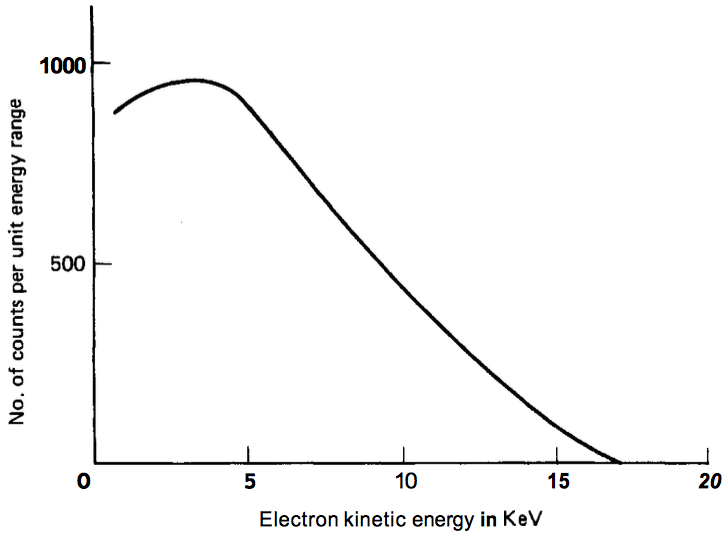
\includegraphics[width=10cm]{ElectronEnergySpectrumBetaDecay.png}
  \caption[Energy spectrum of the electron produced in beta decay.]{Energy spectrum of the electron produced in beta decay \cite{Lewis1970}.}
  \label{fig:BetaDecayEnergy}
\end{figure}

Further indications of the existence of the neutrino were provided by the studies of pion and muon decay by Cecil Powell's group at Bristol in 1947 \cite{Lattes1947-159,Lattes1947-160}.  Topological investigations of the newly discovered $\pi$ meson and its apparent decay into a lighter meson (now known to actually be the muon lepton) appear to hint at the presence of an additional, unknown, daughter particle \cite{Lattes1947-159}.  Furthermore, subsequent studies of the decay of the muons implied a three-body decay involving two unknown final state particles, analogous to the implication of the neutrino in $\beta$-decay by considering the electron energy distribution \cite{Brown1949}.  It seemed a model involving neutrinos could explain these observations and provided more suggestions for the existence of such a particle.

\subsection{Discovery of the Neutrino}\label{NeutrinoDiscovery}

The elegance of Fermi's theory convinced many physicists of the existence of the neutrino but until discovered experimentally it remained a hypothetical `bookkeeping' device.  Given the elusive nature of neutrinos this was not for many years, leading to Pauli famously declaring ``I have done a terrible thing. I have postulated a particle that cannot be detected''.  However, a series of experiments conducted between 1953 and 1956 by Clyde Cowan and Frederick Reines confirmed the hypothesis and were later rewarded with the Nobel Prize in Physics in 1995.  Using the new technology of liquid scintillator detectors \cite{ReinesCowanLiquidScintillation}, they designed an experiment \cite{ReinesCowan1953Proposal} to study the (anti)neutrinos produced in inverse beta decay
\begin{equation}\label{eq:InverseBetaDecay}
  {\bar{\nu}}_e + p \rightarrow e^+ + n
\end{equation}
in the Hanford nuclear reactor in Washington, U.S.A.  Their signal comprised of an initial release of scintillation light when the positron annihilates with an electron, followed a characteristic time later by a gamma ray corresponding to the neutron capture.  The initial results from 1953 \cite{ReinesCowan1953} hinted at an excess over predicted background but the background proved to be much larger than anticipated, mainly due to an underestimation of the effects of cosmic rays.  A second experiment was conducted in 1956, this time 12~m underground and 11~m from the Savannah River reactor in South Carolina.  A neutrino detection rate of 2.9$\pm$0.2 per hour, greater than 20 times the accidental background rate was reported, confirming the previous indications \cite{ReinesCowan1956}.  The experimental discovery of the neutrino was confirmed.  [Bit more description? -- Describe detector, method for detecting positron.]

Ray Davis was also using nuclear reactors to study the interaction rates of neutrinos.  Using a detector comprised of 3000 gallons of carbon tetrachloride (CCl$_4$) also close to the Savannah River reactor, Davis and Harmer searched for the interactions
\begin{equation}\label{eq:DavisAntineutrino}
  \bar{\nu} + \textnormal{Cl}^{37} \rightarrow \textnormal{Ar}^{37} + e^- \hspace{1.5cm} (\bar{\nu} + n \rightarrow p^+ + e^-).
\end{equation}
Since it was known from Reines and Cowan that inverse beta decay
\begin{equation}\label{eq:DavisNeutrino}
  \nu + \textnormal{Cl}^{37} \rightarrow \textnormal{Ar}^{37} + e^- \hspace{1.5cm} (\nu + n \rightarrow p^+ + e^-)
\end{equation}
occurs, this facilitated a comparison between the neutrino and the antineutrino.  They found the interaction shown in Equation~\ref{eq:DavisAntineutrino} occurred at a rate less than 20 times that represented in Equation~\ref{eq:DavisNeutrino}, implying for the first time a difference between neutrinos and antineutrinos \cite{Davis1959}.  This gave rise to the notion of `lepton number' and its conservation in physical interactions.

It was few years before the next chapter in the history of neutrinos, the discovery of the muon neutrino in 1962 at Brookhaven \cite{Danby1962}.  It was noted the apparently permitted decay
\begin{equation}
\mu^- \not\rightarrow e^- + \gamma
\end{equation}
is never observed, inciting the possibility of two distinct neutrinos.  In order to test this, Lederman, Schwarz and Steinberger used a muon neutrino beam to look for two separate interactions:
\begin{align}
  \bar{\nu}_{\mu} + p^+ &\rightarrow \mu^+ + n, \\
  \bar{\nu}_{\mu} + p^+ &\rightarrow e^+ + n.
\end{align}
With only one type of neutrino, each interaction would be expected to occur at around the same rate.  The beam was produced by accelerating protons up to 15 GeV and using a Beryllium target to create secondary mesons, decaying to produce neutrinos with energies up to 1 GeV.  34 muon tracks were detected (with an estimated background from cosmic muons of 5) and no events consistent with electrons were observed.  This remarkable result can only be rivalled by the technological advancements required; it was the first experiment to construct and use an artificial neutrino beam (common to all contemporary long-baseline experiments) and used 13.5~m thick steel from a dismantled battleship in order to ensure only neutrinos arrived at the spark chamber detector.  This discovery was rewarded with the Nobel Prize in 1988.

A third generation of lepton, the $\tau$, was discovered in 1975 by Martin Perl and his team at SLAC \cite{Perl1975}, completing the set of three charged leptons.  They reported 64 events of the form
\begin{equation}
  e^+ + e^- \rightarrow e^{\pm} + \mu^{\mp} + \ge 2 \textnormal{ undetected particles},
\end{equation}
using the energy and angle distributions to predict at least two additional particles.  They claimed `no conventional explanation' could account for these events and proposed the existence of a heavier charged lepton as an intermediate stage:
\begin{equation}
  e^+ + e^- \rightarrow \tau^+ + \tau^- \rightarrow e^{\pm} + \mu^{\mp} + 4\nu.
\end{equation}
The $\tau$ lepton was subsequently characterised by further experiments by the Mark I detector at SLAC \cite{Feldman1977} and by the PLUTO collaboration at DESY \cite{Burmester1977}.  This result heavily implied the existence of an associated neutrino to complete the symmetry observed in the first two lepton couplets.

Further evidence for a third neutrino was provided by four experiments using the Large Electron-Positron Collider (LEP) at CERN in 1989 which were studying the production of the newly discovered Z$^0$ boson \cite{DeCamp1989,Adeva1989,Akrawy1989,Aarnio1989}.  The width $\Gamma_Z$ of the Z$^0$ resonance is dependent on the partial widths relating to final state charged leptons, hadrons and neutrinos;
\begin{equation}
  \Gamma_Z = N_{\nu} \Gamma_{\nu} + 3 \Gamma_{ee} + \Gamma_{\mathrm{hadron}},
\end{equation}
where $N_{\nu}$ is the number of light ($m_{\nu} \le \frac{m_Z}{2}$) active neutrinos.  Figure~\ref{fig:LEPZ0Resonance} shows this resonance for a range of $N_{\nu}$ hypotheses; fitting to the data yields a value of $2.984 \pm 0.008$ neutrino flavours \cite{Schael2006}.

\begin{figure}
  \centering
  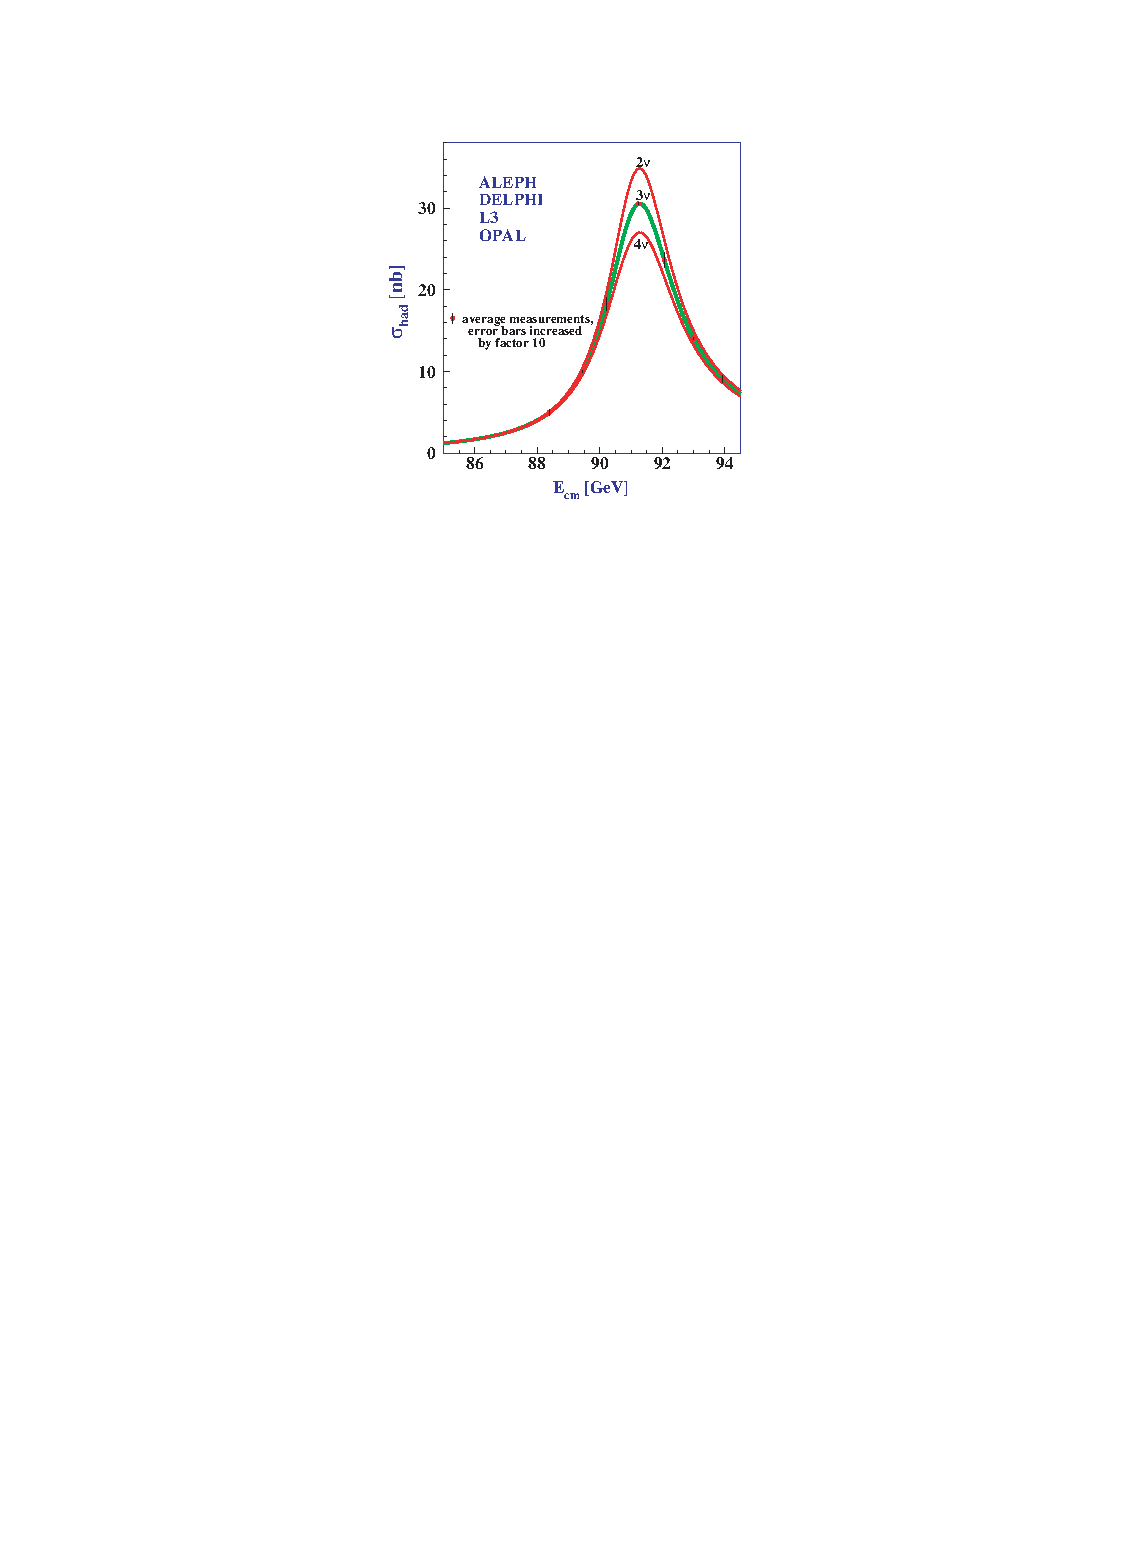
\includegraphics[width=12cm]{LEPZ0Resonance.pdf}
  \caption[Measurements of the hadron production cross-section around the Z resonance.]{Measurements of the hadron production cross-section around the Z resonance.  The curves indicate the predicted cross-section for two, three and four neutrino species with SM couplings and negligible mass.  Taken from \cite{Schael2006}.}
  \label{fig:LEPZ0Resonance}
\end{figure}

The extremely precise measurement reported by the LEP experiments was enough for many physicists to claim indisputable evidence for the existence of the tau neutrino; it was partly for this reason that its experimental discovery was not until 25 years after the addition of the $\tau$ lepton to the Standard Model.  However, in 2000 the DONUT (Direct Observation of NuTau) experiment at Fermilab, IL, U.S.A. finally reported direct detection of the tau neutrino \cite{Kodama2001}.  As its name suggests, DONUT was designed specifically for the purpose of finding the third neutrino.  It did this by identifying the $\tau$ as the only lepton at the interaction vertex from a $\nu_{\tau}$ beam created by firing 800 GeV protons from the Tevatron at a tungsten beam dump.  The mean energy of the $\nu_{\tau}$s detected at the emulsion target 36~m downstream was 111~GeV, produced by the decay of a $D_S$ meson to a $\tau$ lepton and a $\bar{\nu}_{\tau}$ neutrino followed by the decay of the $\tau$ to a $\nu_{\tau}$.  Four events were found, above a predicted background of $0.34\pm0.05$, consistent with the Standard Model description of the tau neutrino.

\subsection{The Solar Neutrino Problem}\label{SolarNeutrinoProblem}

It has been known since the 1930s, when Hans Bethe started developing the ideas of stellar nucleosynthesis \cite{Bethe1939}, that an abundance of electron neutrinos is created as byproducts of the nuclear processes powering the Sun.  The Standard Solar Model (SSM), established by John Bahcall in 1968 \cite{Bahcall1968}, explains the nuclear fusion processes responsible for powering stars.  For stars the size of the Sun, this is dominated by the \textit{proton-proton chain}; heavier stars follow the \textit{CNO cycle}.  Figure~\ref{fig:SolarNeutrinoCycles} shows the energy spectra of neutrinos released during reactions occurring during both chains.

\begin{figure}
\centering
  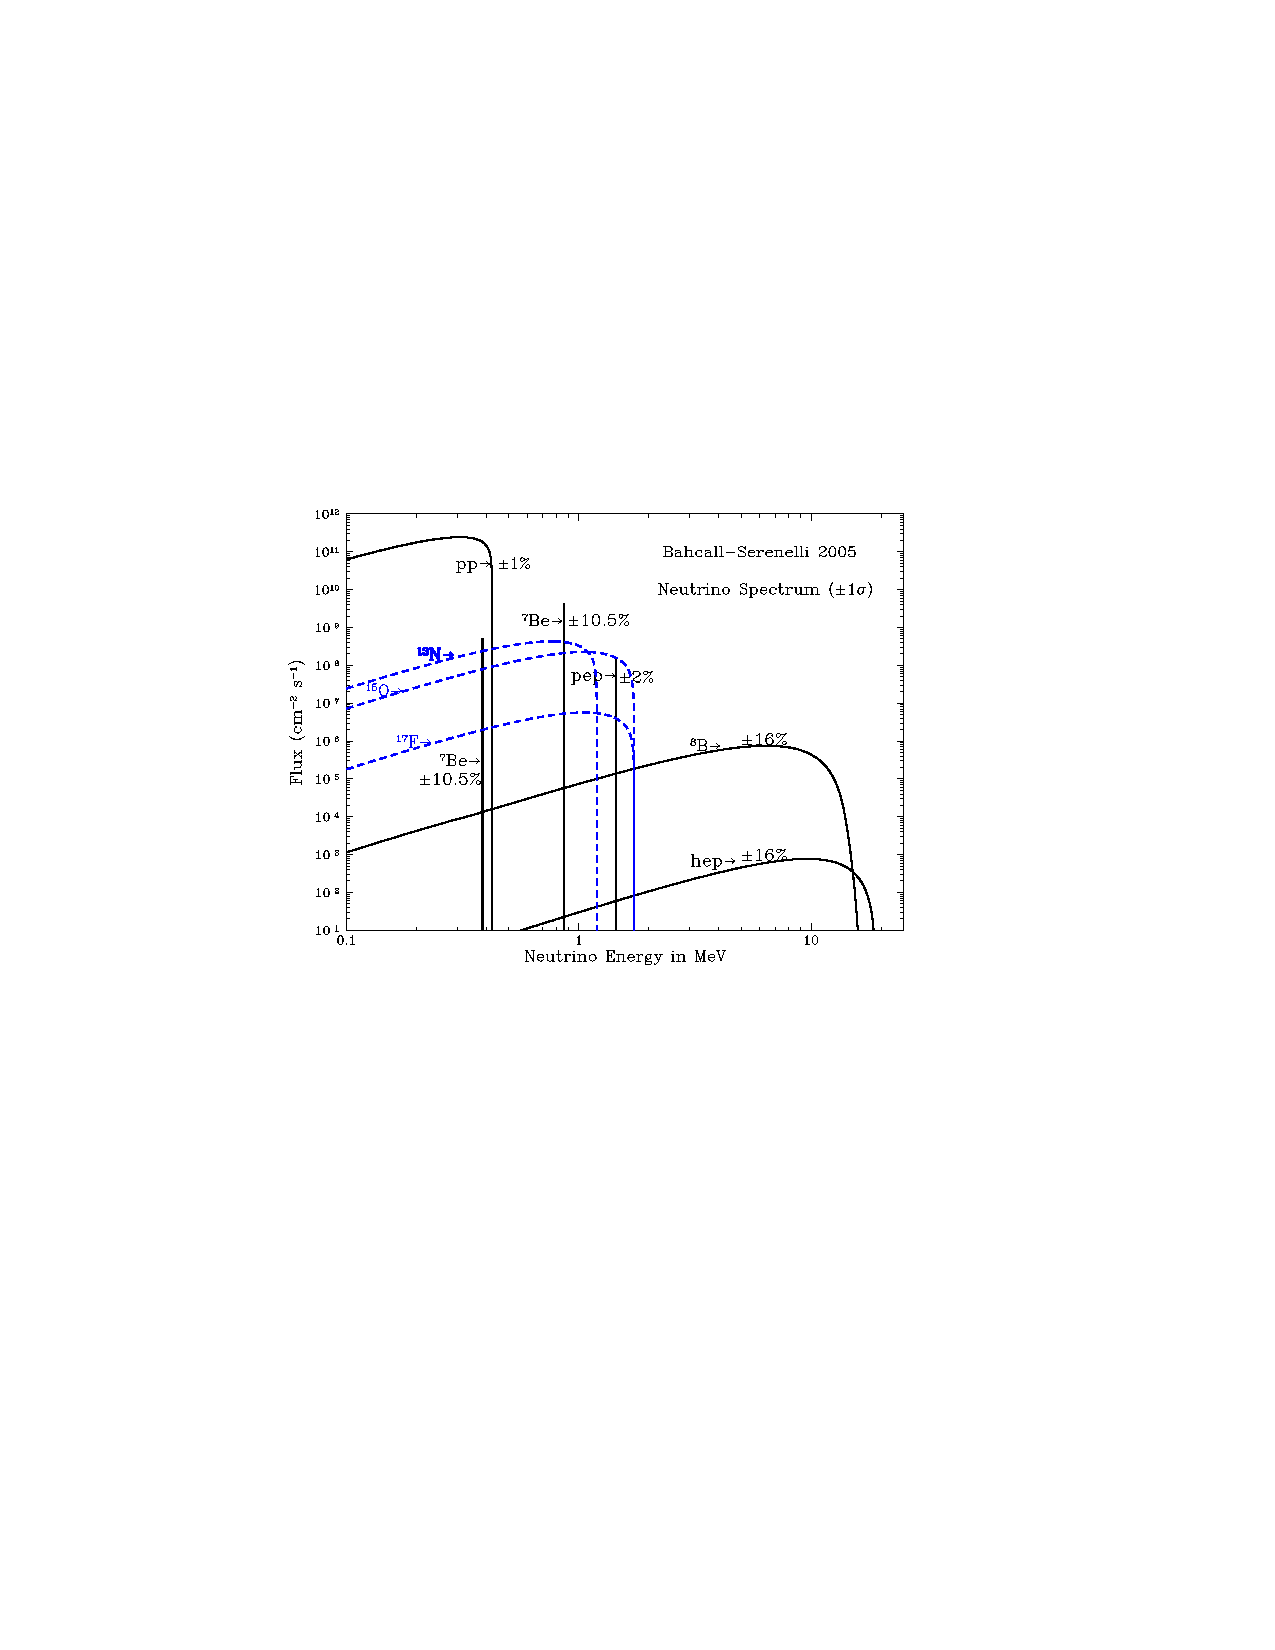
\includegraphics[width=12cm]{SolarNeutrinoCycles.pdf}
  \caption{Solar neutrino energy spectra as predicted by the Standard Solar Model \cite{Bahcall2005}.  The solid lines represent neutrinos produced during the p-p chain and dashed line represent neutrinos from the CNO cycle.  Each spectrum illustrates a particular reaction during the process of a given chain.}
  \label{fig:SolarNeutrinoCycles}
\end{figure}

Ray Davis, in collaboration with Bahcall, conducted the first experiment to detect these solar neutrinos in 1968.  Using a similar detection technique to his previous experiments, Davis used a 380~m$^3$ tank of tetrachloroethene (C$_2$Cl$_4$) to detect neutrinos via the inverse beta decay reaction detailed in Equation~\ref{eq:DavisNeutrino}.  Given the threshold for this reaction is 0.814 MeV, the main sources of neutrinos probed by this experiment were Be$^7$ and B$^8$.  In order to eliminate backgrounds from cosmic rays, Davis constructed his experiment 4850~ft underground at the Homestake mine near Lead, SD, U.S.A.  It is worth noting, in a pleasing neutrino-full-circle, this is exactly where the far detector for the DUNE experiment will be housed.  The Davis Homestake experiment ran for 25 years but the results obtained \cite{Cleveland1995} disagreed quite strongly with the SSM \cite{Bahcall1995}, consistently measuring solar electron neutrinos at a rate around a third of that predicted by the model.  This became known as the `solar neutrino problem', and Davis was awarded the Nobel Prize for his work on this famous experiment in 2002.

The subsequent radiochemical experiments SAGE (from 1990) and GALLEX (from 1991) were sensitive to the large flux of \textit{pp} neutrinos by utilising a Ga$^{71}$ target and the lower threshold reaction
\begin{equation}
\nu + \textnormal{Ga}^{71} \rightarrow \textnormal{Ge}^{71} + e^-.
\end{equation}
These experiments also reported `missing' neutrinos, determining capture rates of $66.6^{+6.8+3.8}_{-7.1-4.0}$~SNU (SAGE) \cite{Abdurashitov1994} and $77.5\pm6.2^{+4.3}_{-4.7}$~SNU (GALLEX) \cite{Anselmann1992}, disagreeing with the SSM prediction of 130~SNU \cite{Hampel1999}.  There appeared to be a problem -- either the SSM was incomplete and incorrectly over-predicted the amount of electron neutrinos or hints of new physics were beginning to appear in the experiment data.

\subsection{The Atmospheric Neutrino Anomaly}\label{sec:AtmosphericNeutrinoAnomaly}

Another abundant source of natural neutrinos come from cosmic rays interacting with the upper atmosphere and producing `atmospheric neutrinos', typically via the interactions \cite{Gaisser1990}
\begin{align}
  \pi^+ \rightarrow \mu^+ + \nu_{\mu}, &\hspace{1.5cm} \mu^- \rightarrow e^- + \bar{\nu}_e + \nu_{\mu} \\
  \pi^- \rightarrow \mu^- + \bar{\nu}_{\mu}, &\hspace{1.5cm} \mu^+ \rightarrow e^+ + \nu_e + \bar{\nu}_{\mu}.
\end{align}
Since the decay lengths and kinematics are well known, the predicted ratio of muon to electron neutrinos can be calculated to a good accuracy.  This ratio can be compared to an experimentally determined ratio and analysed as a measure of the efficacy of the model.

It was first noticed as early as the late 1970s by experiments designed to search for nucleon decay predicted by the then-popular Grand Unified Theories that the measured flux did not correspond to that predicted by the theory.  The IMB \cite{Haines1986} and Kamioka \cite{Hirata1988} experiments, whilst measuring the atmospheric neutrino flux as an important background for nucleon decay, both noticed deficiencies in the ratio between muon and electron neutrinos compared to that predicted by the models.  These experiments utilised large tanks of pure water surrounded by Photo-Multiplier Tubes (PMTs) to detect neutrinos via the Cherenkov radiation created by their charged leptonic daughter particles.  Using ring-imaging techniques, it is possible to distinguish between electron-like and muon-like events and therefore identify the flavour of the incoming neutrino.  The problem implied by these measurements is known as the `atmospheric neutrino anomaly'.

Various other experiments over the following twenty years also reported similar measurements, suggesting an excess of electron neutrinos over prediction, a deficit in the number of muon neutrinos, or both.  Results from numerous experiments are shown in Figure~\ref{fig:AtmosphericNeutrinoAnomaly}.  Most experiments report a discrepancy, with its size seemingly dependent on the energy region being studied.  The experiments reporting a ratio consistent with one were much smaller than the others, and with more statistics they also started observing similar effects.  This anomaly, along with the issue of the solar neutrino problem, strongly hinted at a problem with our understanding of neutrino physics.  This is be discussed in detail in the Section~\ref{sec:NeutrinoOscillations}.

\begin{figure}
  \centering
  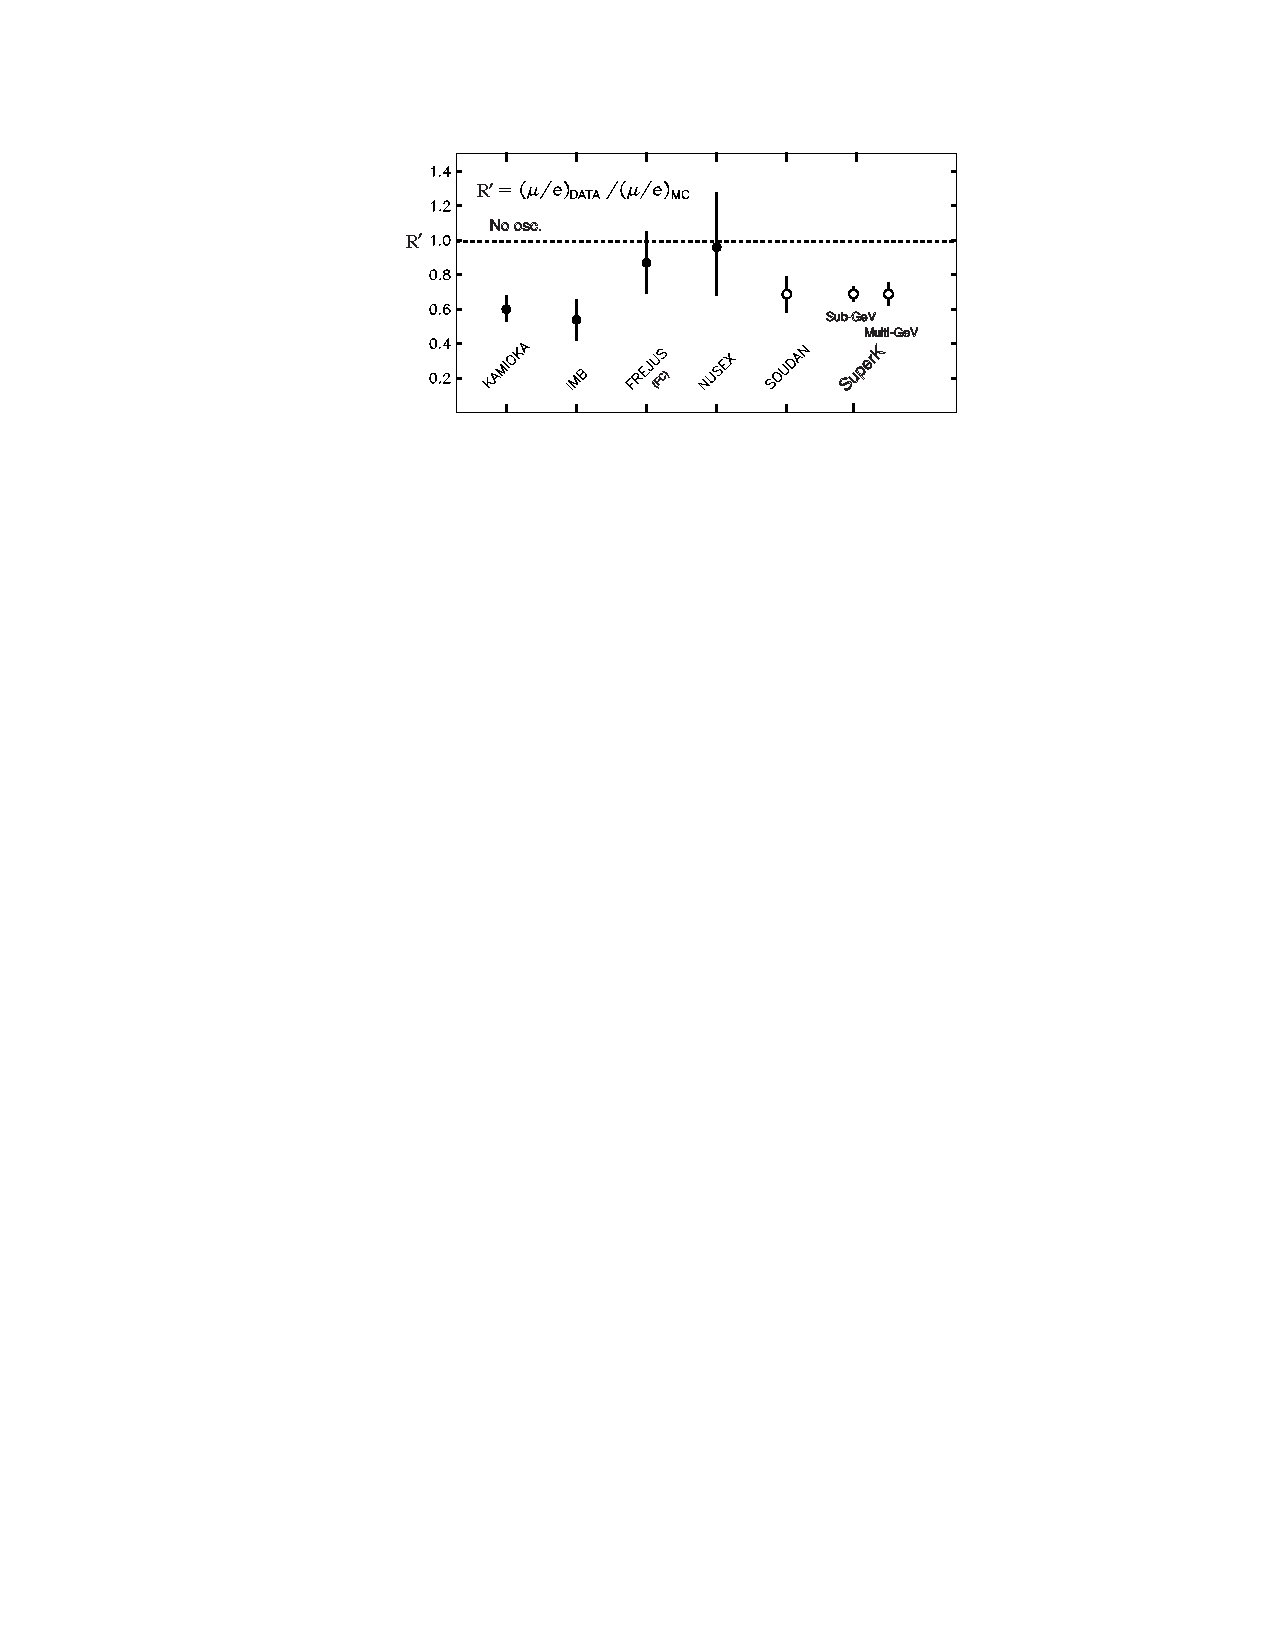
\includegraphics[width=12cm]{AtmosphericNeutrinoAnomaly.pdf}
  \caption{The double ratio \textit{R} of muon to electron neutrino events showing data divided by expectation \cite{Mann1999}.  Various underground atmospheric neutrino detectors are shown.}
  \label{fig:AtmosphericNeutrinoAnomaly}
\end{figure}

%----------------------------------------------------------------------------------------------------------------------------------------------------------------------------
\section{Neutrino Oscillations}\label{sec:NeutrinoOscillations}

The concept of neutrino oscillations involves the changing of the flavour of a neutrino as it propagates through time and space; a neutrino created in a certain flavour has a non-zero probability of being later detected in a different flavour state.  It was first postulated as an explanation of the Solar Neutrino Problem by Pontecorvo in 1968 \cite{Pontecorvo1968,Pontecorvo1969}, having initially proposed the phenomenon in 1957 as an analogy to $\textnormal{K}^0 \rightarrow \widetilde{\textnormal{K}}^0$ transition in the quark sector \cite{Pontecorvo1957}.  It offers an elegant solution to both the solar neutrino problem and the atmospheric neutrino anomaly by explaining where the `missing' neutrinos had gone; it is possible they had simply `oscillated' to a different flavour and therefore would not be detected as expected.

\subsection{The Evidence for Neutrino Oscillations}\label{sec:EvidenceNeutrinoOscillations}

Whilst there was speculation that neutrino oscillations may be the explanation behind the issues observed in the data much sooner \cite{Casper1991,BeckerSzendy1992}, definite proof was not provided until the late 1990s.  In many ways, the story of neutrino physics, from the initial observations of the Solar Neutrino Problem and the Atmospheric Neutrino Anomaly, through the speculation and theoretical developments, to the eventual proof, can be considered a triumph for the scientific method.

The Kamiokande and Super-Kamiokande experiments in Japan (upgrades from the Kamioka experiment noted previously) and the SNO experiment in Sudbury, Canada produced the results which showed indisputable evidence for neutrino oscillations and provided explanations for all previous discrepancies observed.  This result was monumental and the work of both collaborations was rewarded in 2015 when the Nobel Prize was awarded to T. Kajita and A. McDonald, from Super-Kamiokande and SNO respectively.

\subsubsection{Super-Kamiokande and the Atmospheric Sector}\label{sec:SuperKamiokande}

In 1994, the Kamiokande experiment produced results which hinted at an angular dependence for the $R$-ratio deficit, implying a dependence on neutrino travel distance \cite{Kamiokande1994}.  This result can be explained by invoking neutrino oscillations since the probability of oscillation is influenced by the propagation distance; its significantly larger successor, Super-Kamiokande, was constructed in order to make precise measurements of this phenomenon.  Super-Kamiokande is located 1000~m underground and contains an inner detector consisting of 22.5~kton fiducial volume of pure water contained within a large stainless steel cylinder (37~m high, 34~m diameter) and surrounded by 13142 20-inch photo-multipliers.  With 40\% coverage, the photocathodes extended over nearly an acre and provided ten times more pixels than any other experiment at the time.  Its results in 1998 confirmed the earlier angular dependence findings of Kamiokande, Figure~\ref{fig:SuperKamiokandeDirection}, and also considered the data as a function of neutrino energy and propagation distance, as shown in Figure~\ref{fig:SuperKamiokandeLE}.  The observed effects disagreed with a view of non-oscillating atmospheric neutrinos but were entirely consistent with a two-flavour oscillation model, $\nu_{\mu} \rightarrow \nu_{\tau}$.  This resulted in the famous published claim for the experimental discovery of neutrino oscillations \cite{SuperKamiokande1998}.

\begin{figure}
  \centering
  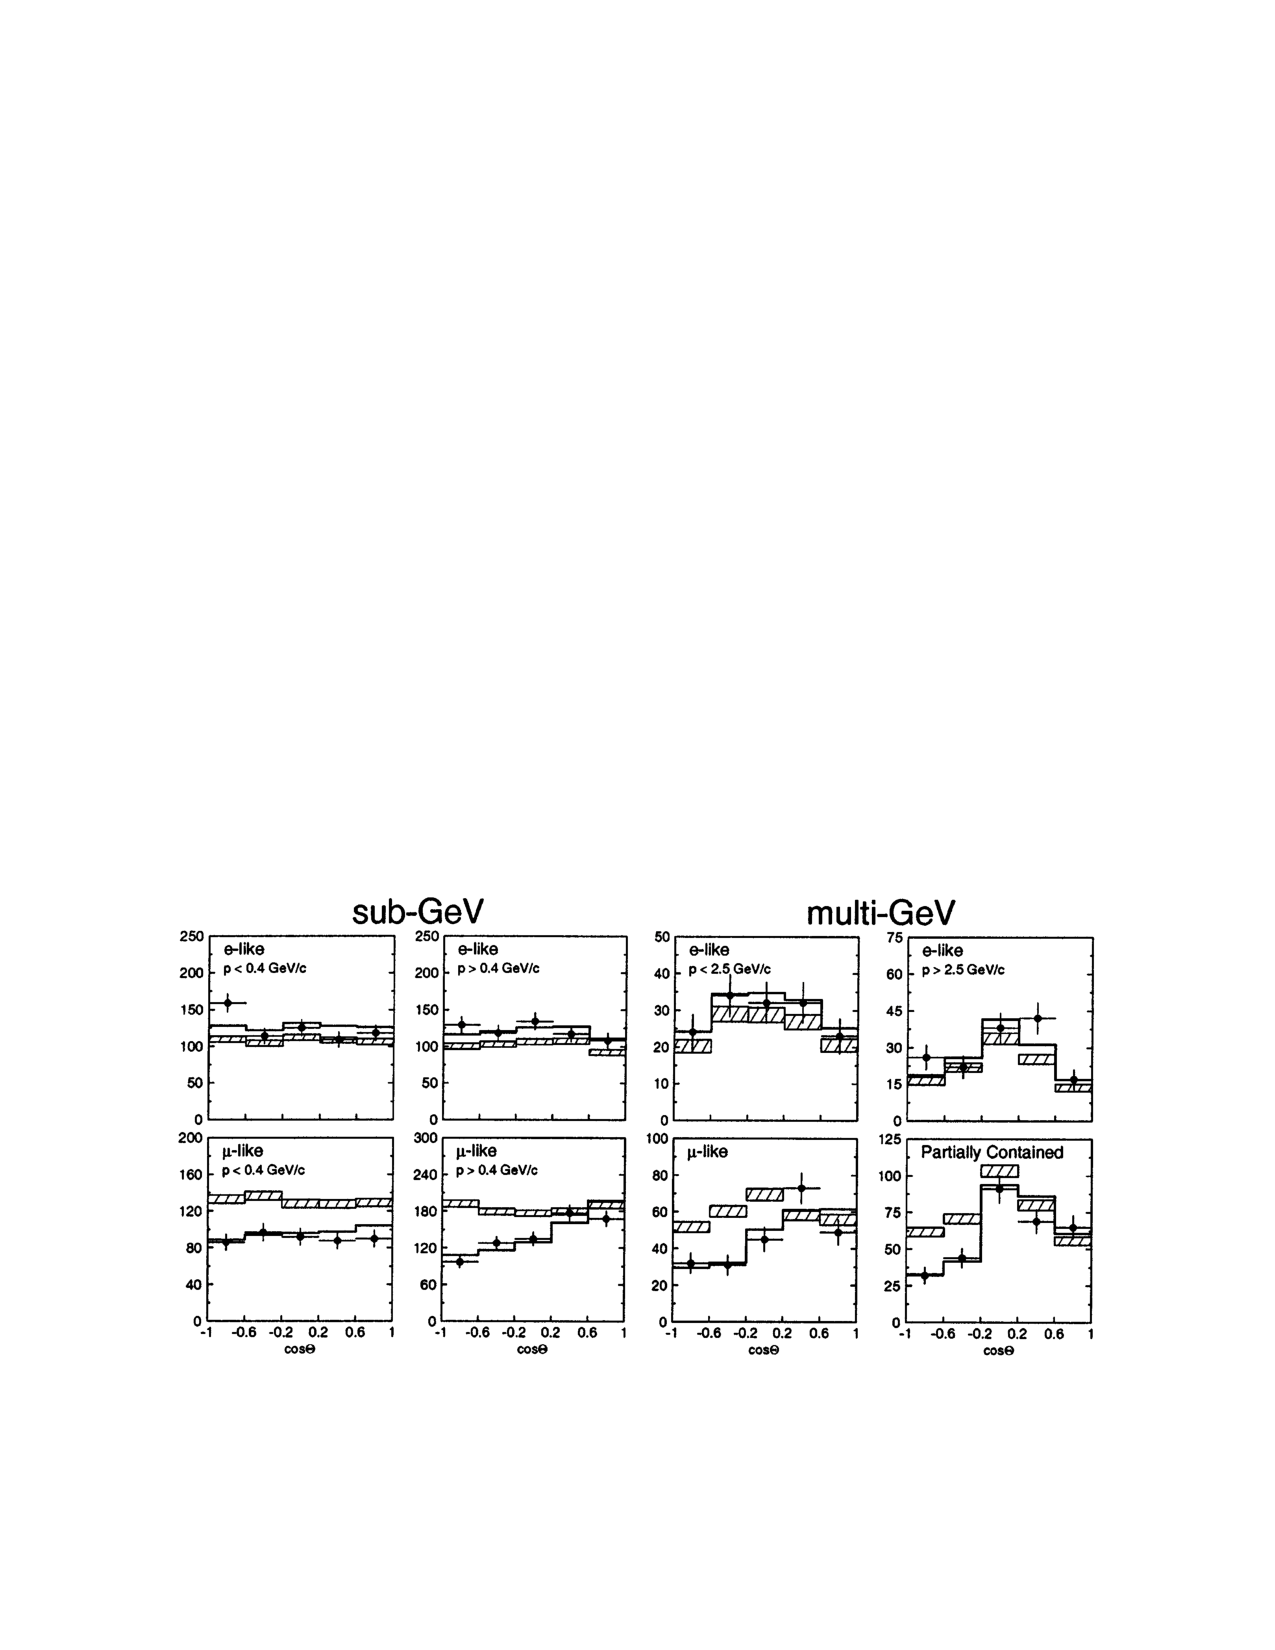
\includegraphics{SuperKamiokandeDirection.pdf}
  \caption{Zenith angle distributions of $\mu$-like and $e$-like events for sub-GeV and multi-GeV data sets.  Upward-going particles have $\cos{\Theta} < 0$ and downward-going particles have $\cos{\Theta} > 0$.  The hatched region shows the Monte Carlo expectation for no oscillations and the bold line is the best-fit expectation for $\nu_{\mu}\rightarrow\nu_{\tau}$ oscillations.  Taken from \cite{SuperKamiokande1998}.}
  \label{fig:SuperKamiokandeDirection}
\end{figure}

\begin{figure}
  \centering
  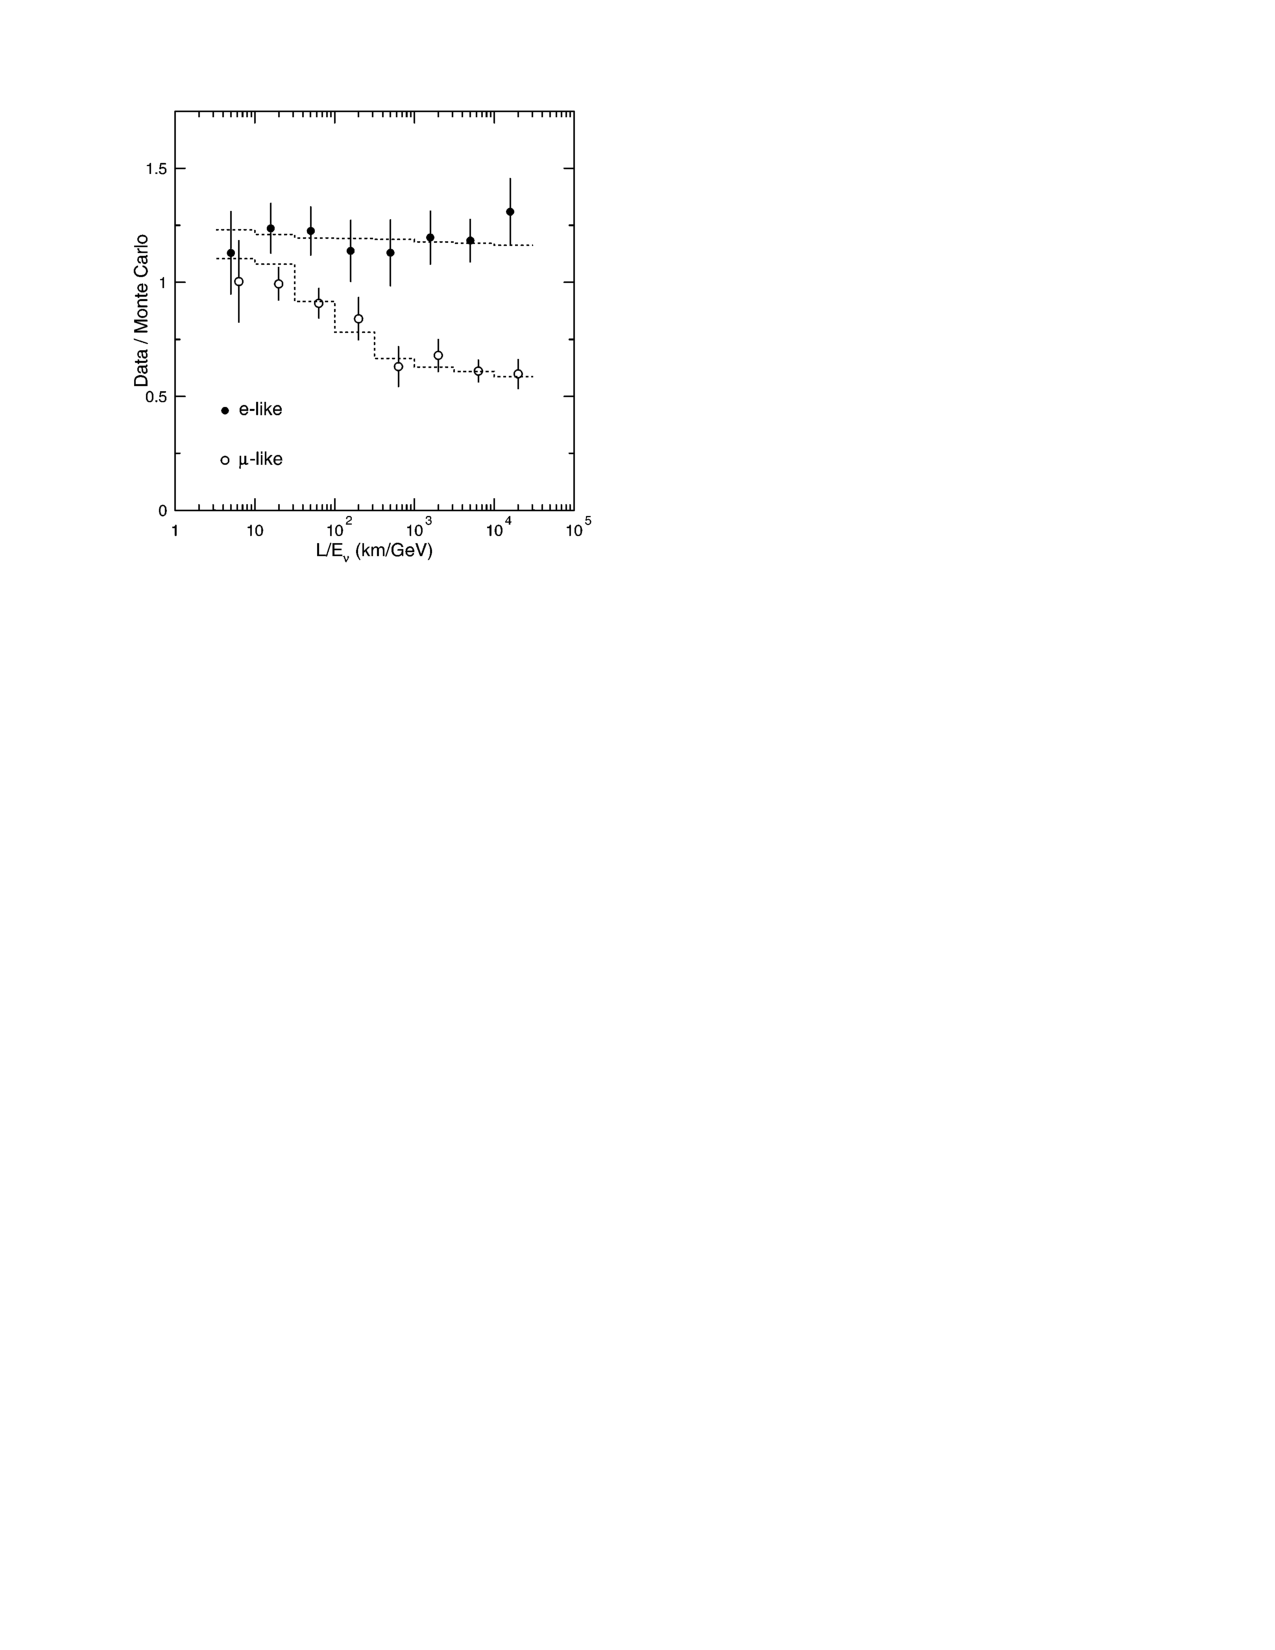
\includegraphics{SuperKamiokandeLE.pdf}
  \caption{The ratio of the number of data events to Monte Carlo events in the absence of oscillations as a function of reconstructed $L/E_{\nu}$.  The dashed lines show the expected shape for $\nu_{\mu}\rightarrow\nu_{\tau}$ oscillations.  Taken from \cite{SuperKamiokande1998}.}
  \label{fig:SuperKamiokandeLE}
\end{figure}

\subsubsection{SNO and the Solar Sector}\label{sec:SNO}

After the Super-Kamiokande results, it was clear that neutrino oscillations would probably also explain the deficit of electron neutrinos observed by solar neutrino experiments.  It took a few years until the Sudbury Neutrino Observatory (SNO) in Canada provided some quite brilliant evidence of this in 2002 \cite{SNO2002}.

SNO was a water Cherenkov detector, like Super-Kamiokande, but used heavy water (D$_2$O) as a detector medium.  The water is contained in a 12~m acrylic spherical shell and surrounded by 9456 photomultipliers at a depth of 6010~m water equivalent.  The use of heavy water facilitated sensitivity to other neutrino interaction channels not accessible by Super-Kamiokande via the charge current (CC), neutral current (NC) and elastic scattering (ES) interactions;
\begin{align}
  \nu_e + d &\rightarrow p + p + e^- &\textnormal{(CC)} \\
  \nu_x + d &\rightarrow p + n + \nu_x &\textnormal{(NC)} \\
  \nu_x + e^- &\rightarrow \nu_x + e^- &\textnormal{(ES)}.
\end{align}
The CC channel is sensitive exclusively to electron neutrinos, whilst the other two are accessible by neutrinos of any flavour.  This allowed for the first time a simultaneous measurement of the total neutrino interaction rate as well as the electron neutrino interaction rate.  The observations of SNO were the smoking gun for neutrino oscillations; the total measured flux for all neutrinos, $\phi_{\textnormal{NC}}^{\textnormal{SNO}} = 6.42\pm1.57\textnormal{~(stat.)}^{+0.55}_{-0.58}\textnormal{~(sys.)}$~cm$^{-2}$s$^{-1}$, agreed excellently with the electron neutrino flux predicted by the SSM, $\phi^{\textnormal{SSM}} = 5.05^{+1.01}_{-0.81}$~cm$^{-2}$s$^{-1}$.  However, the measured electron neutrino flux was around a third lower, $\phi_e^{\textnormal{SNO}} = 1.76\pm0.05\textnormal{~(stat.)}\pm0.09\textnormal{~(sys.)}$~cm$^{-2}$s$^{-1}$, consistent with previous measurements from the radiochemical experiments.  The evidence seems conclusive: the solar models are correct and the neutrinos are not disappearing; there are simply changing their flavour state.  A summary plot showing all solar neutrino experiments up until this point is depicted in Figure~\ref{fig:SolarNeutrinoFluxes} \cite{Bahcall2005Fluxes}.

\begin{figure}
  \centering
  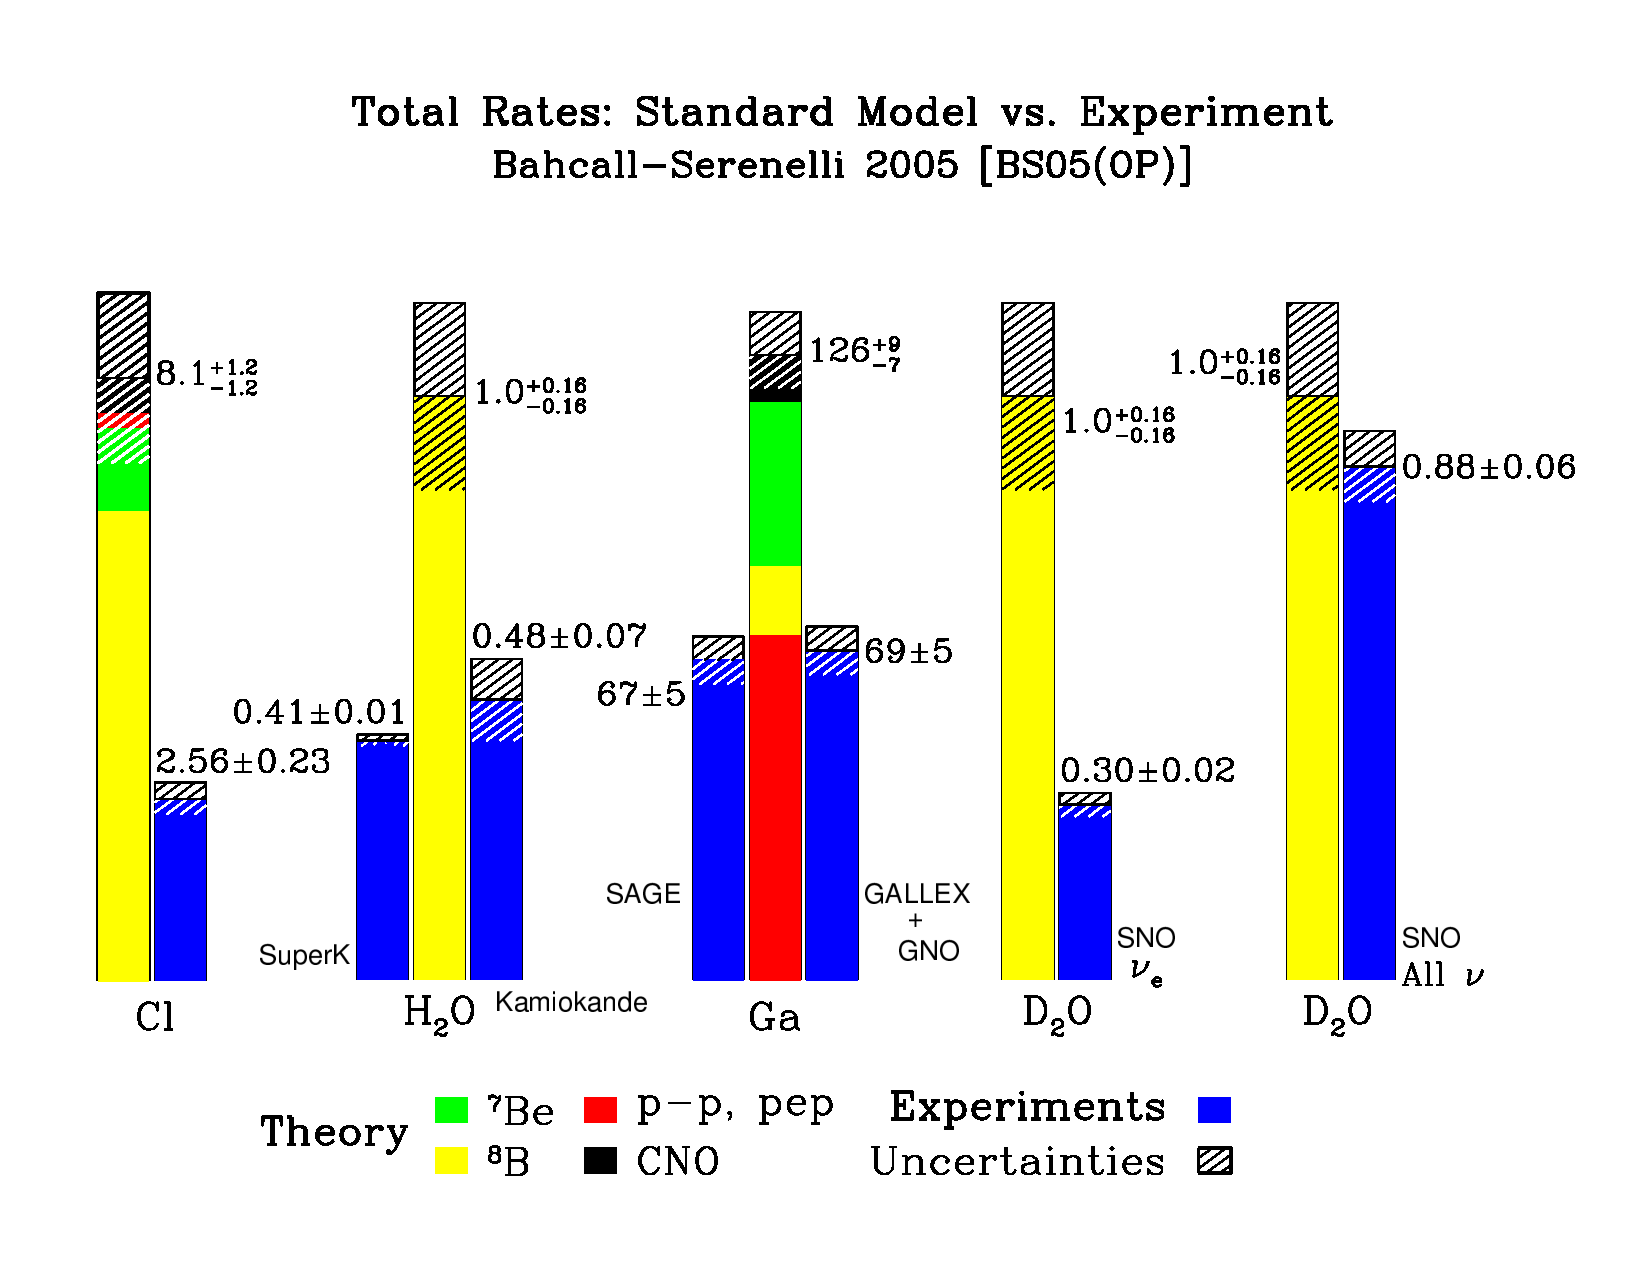
\includegraphics[width=16cm]{SolarNeutrinoFluxes.pdf}
  \caption{Comparison of the predictions of the neutrino fluxes from the Standard Solar Model with measured rates from a variety of solar neutrino experiments.  The results of SNO (D$_2$O target, right two comparisons) show that the expected flux is observed, but not necessarily as electron neutrinos.  This shows conclusively the oscillatory nature of neutrinos.}
  \label{fig:SolarNeutrinoFluxes}
\end{figure}

\subsection{Vacuum Oscillations}\label{sec:VacuumOscillations}

The theory of neutrino oscillations is basically the quantum mechanics of mixed states and was developed on top of Pontecorvo's work by Ziro Maki, Masami Nakagawa and Shoichi Sakata \cite{MNS1962}.  If the neutrino flavour states can spontaneously convert from one to another, none can be considered as eigenfunctions of the Hamiltonian.  The true stationary states are the \textit{mass eigenstates} ($\nu_1$, $\nu_2$, $\nu_3$), of which the flavour states ($\nu_e$, $\nu_{\mu}$, $\nu_{\tau}$) can be considered linear superpositions:
\begin{equation}
  \begin{pmatrix}
    \nu_e \\
    \nu_{\mu} \\
    \nu_{\tau} \\
  \end{pmatrix}
  =
  U^*_{\textnormal{PMNS}}
  \begin{pmatrix}
    \nu_1 \\
    \nu_2 \\
    \nu_3 \\
  \end{pmatrix},
  \label{eq:FlavourMassStates}
\end{equation}
where $U_{\textnormal{PMNS}}$ is the PMNS mixing matrix which described the flavour composition of each of the mass eigenstates, and vice versa.  If the PMNS matrix were diagonal, each flavour state would correspond to a single mass state and oscillations would not occur.

Just as the flavour states are a superposition of mass states
\begin{equation}\label{eq:FlavourSuperposition}
  \ket{\nu_{\alpha}} = \sum_i U^*_{\alpha i} \ket{\nu_i},
\end{equation}
the mass states can also be considered a superposition of flavour states
\begin{equation}\label{eq:MassSuperposition}
  \ket{\nu_i} = \sum_{\alpha} U_{\alpha i} \ket{\nu_{\alpha}}.
\end{equation}

For the three neutrino case, the PMNS matrix, decomposed into its three axial rotations, can be expressed as
\begin{equation}
  U_{\alpha i} \equiv
  \underbrace{
    \begin{pmatrix}
      1 & 0 & 0 \\
      0 & c_{23} & s_{23} \\
      0 & -s_{23} & c_{23} \\
    \end{pmatrix}
  }_{\textnormal{`Atmospheric' term}}
  \underbrace{
    \begin{pmatrix}
      c_{13} & 0 & e^{-i\delta} s_{13} \\
      0 & 1 & 0 \\
      -e^{-i\delta} s_{13} & 0 & c_{13} \\
    \end{pmatrix}
  }_{\textnormal{`Accelerator' or `Reactor' term}}
  \underbrace{
    \begin{pmatrix}
      c_{12} & s_{12} & 0 \\
      -s_{12} & c_{12} & 0 \\
      0 & 0 & 1 \\
    \end{pmatrix}
  }_{\textnormal{`Solar' term}}
  ,
  \label{eq:PMNS}
\end{equation}
where $c_{ij} \equiv \cos{(ij)}$, $s_{ij} \equiv \sin{(ij)}$ and $\delta$ is a CP-violating phase factor.  Each axial component is often referred to by the means with which they are studied, as shown in Equation~\ref{eq:PMNS}.

The weak interaction couples to the flavour eigenstates so neutrinos are always created and detected as flavour states.  However, they propagate as mass states since it is these which are eigenstates of the Hamiltonian.  Due to the misalignment of the flavour and mass states, oscillations can be shown to occur.  A neutrino created with flavour $\alpha$ is a superposition of all the mass states (Equation~\ref{eq:FlavourSuperposition}).  These states propagate as a plane wave, evolving in time and space such that
\begin{equation}\label{eq:MassTimeEvolution}
  \ket{\nu_i(x,t)} = \ket{\nu_i (0)} e^{-i \textbf{x} \cdot \textbf{p}},
\end{equation}
where \textbf{x} and \textbf{p} are the 4-position and 4-momentum of the neutrino respectively.  From Equations~\ref{eq:FlavourSuperposition} and~\ref{eq:MassTimeEvolution}, the evolution of the flavour states over space and time is therefore
\begin{align}
  \nonumber \ket{\nu_{\alpha}(x,t)} &= \sum_i U_{\alpha i}^* \ket{\nu_i (x,t)} \\
  \label{eq:FlavourTimeEvolution} &= \sum_i U_{\alpha i}^* e^{-i \textbf{x} \cdot \textbf{p}} \ket{\nu_i(0)} .
\end{align}
In the ultra-relativistic limit, the mass of the neutrino is negligible compared to its momentum ($m_i \ll \vec{p}$) and $\vec{x} \approx ct$;
\begin{align}
  \label{eq:RelativisticEnergy} E_i &= \sqrt{|\vec{p}|^2+m_i^2} = \vec{p}\sqrt{1+\frac{m_i^2}{|\vec{p}|^2}} \approx \vec{p}+\frac{m_i^2}{2\vec{p}} \\
  \label{eq:RelativisticEnergyMomentum} \textbf{x}\cdot\textbf{p} &= E_i t - \vec{x}\cdot\vec{p} = \vec{p}\cdot t + \frac{m_i^2}{2\vec{p}}t - \vec{x}\cdot\vec{p} \approx \frac{m_i^2}{2\vec{p}}\vec{x} = \frac{m_i^2}{2p}x ,
\end{align}
assuming the neutrino displacement is in the direction of its momentum and using natural units ($c \equiv \hbar \equiv 1$).  Thus, using Equations~\ref{eq:FlavourTimeEvolution}, \ref{eq:RelativisticEnergyMomentum} and~\ref{eq:MassSuperposition},
\begin{align}
  \nonumber \ket{\nu_{\alpha}(x,t)} &= \sum_i U_{\alpha i}^* e^{-i \frac{m_i^2}{2p} x} \ket{\nu_i (0)} \\
  \label{eq:FlavourEvolution} &= \sum_i \sum_{\beta} U_{\alpha i}^* e^{-i \frac{m_i^2}{2p} x} U_{\beta i} \ket{\nu_{\beta}}.
\end{align}

The probability of a neutrino created in flavour state $\alpha$ being observed in flavour $\beta$ can be determined from Equation~\ref{eq:FlavourEvolution}
\begin{align}
  P(\alpha \rightarrow \beta) &= |\braket{\nu_{\alpha}}{\nu_{\beta}(x,t)}|^2 \\
  &= \left[ \sum_i U_{\alpha i} e^{i \frac{m_i^2}{2p} x} U_{\beta i}^* \right] \left[ \sum_j U_{\alpha j}^* e^{-i \frac{m_j^2}{2p} x} U_{\beta j} \right] \\
  &= \sum_{i,j} U_{\alpha i} U_{\alpha j}^* U_{\beta j} U_{\beta i}^* e^{i \frac{m_i^2-m_j^2}{2p} x},
\end{align}
and is observed to be dependent on the neutrino momentum, the difference between the squared masses of the flavour states, the propagation distance and the relative mixing of the two flavour states encoded in the matrix elements $U$.

An accelerator based neutrino experiment, such as DUNE, will typically use a $\nu_{\mu}$-dominated beam and look for \textit{muon neutrino disappearance} ($P(\nu_{\mu}\rightarrow \nu_{\mu})$) and \textit{electron neutrino appearance} ($P(\nu_{\mu}\rightarrow \nu_e)$).  In this case, also in the relativistic limit, the relevant appearance and disappearance probabilities can be approximated, respectively, as
\begin{align}
  \label{eq:ElectronNeutrinoAppearance} P(\nu_{\mu} \rightarrow \nu_e) &\approx \sin^2{2\theta_{13}} \sin^2{\theta_{23}} \sin^2 {\left( 1.27 \frac{\Delta m_{13}^2 L}{E} \right)} \\
  \label{eq:MuonNeutrinoDisappearance} P(\nu_{\mu} \rightarrow \nu_{\mu}) &\approx 1 - \cos^4{\theta_{13}} \sin^2{2\theta_{23}} \sin^2{ \left( 1.27 \frac{\Delta m_{23}^2 L}{E} \right) },
\end{align}
where $\Delta m_{ij}^2 \equiv m_i^2-m_j^2$ is the \textit{mass squared splitting} in eV, $L$ is the distance propagated in km and $E$ is the neutrino energy in GeV.

From these equations, it can be seen the important controllable parameters relevant for observing oscillations are the neutrino energy and the distance they travel.  An experiment will typically choose a ratio $L/E$ which will attempt to maximise the effect of oscillations in order to make precision measurements.

\subsection{Matter Effects}\label{sec:MatterEffects}

The oscillations considered thus far are \textit{vacuum oscillations} which occur due to the mixing of the neutrino mass and flavour states.  Whilst directly confirming the oscillation of solar neutrinos, the SNO experiment (along with every other solar neutrino experiment) reported more oscillations than can be explained using just the vacuum oscillation model discussed in Section~\ref{sec:VacuumOscillations} \cite{Bahcall2002,Smirnov2003}.  When neutrinos propagate through matter, an additional potential can be shown to also produce oscillations, which would occur even in the case of massless neutrinos (as long as mixing occurs).  Since solar neutrinos travel through dense matter before exiting the Sun, it is possible these matter effects explained above could explain this discrepancy.

Coherent scattering (scattering in which the neutrino state is unchanged) due to interactions with the medium cause neutrinos travelling through matter to feel a potential.  As normal matter is composed of electrons, rather than their heavier counterparts muons and taus, electron neutrinos are affected more by this potential.  The mechanism for this is demonstrated in Figure~\ref{fig:MatterEffects}.  This gives rise to an additional effective mass splitting between the electron neutrino and the other flavours and therefore results in the possibility of oscillations \cite{Wolfenstein1978}.  Due to the density of the Sun and the neutrino energies, the neutrinos actually feel a resonance which causes their oscillation probability to become dramatically higher than the vacuum oscillation probabilities.  This is known as the Mikheev-Smirnov-Wolfenstein (MSW) effect \cite{MS1985,MS1986}.  It is worth pointing out at this point that, since normal matter is composed of electrons and not positrons, this effect is also different for $\nu_e$s and $\bar{\nu}_e$s; the importance of this becomes apparent when considering the additional effects of CP violation.

\begin{figure}
  \centering
  \begin{subfigure}{0.48\linewidth}
    \centering
    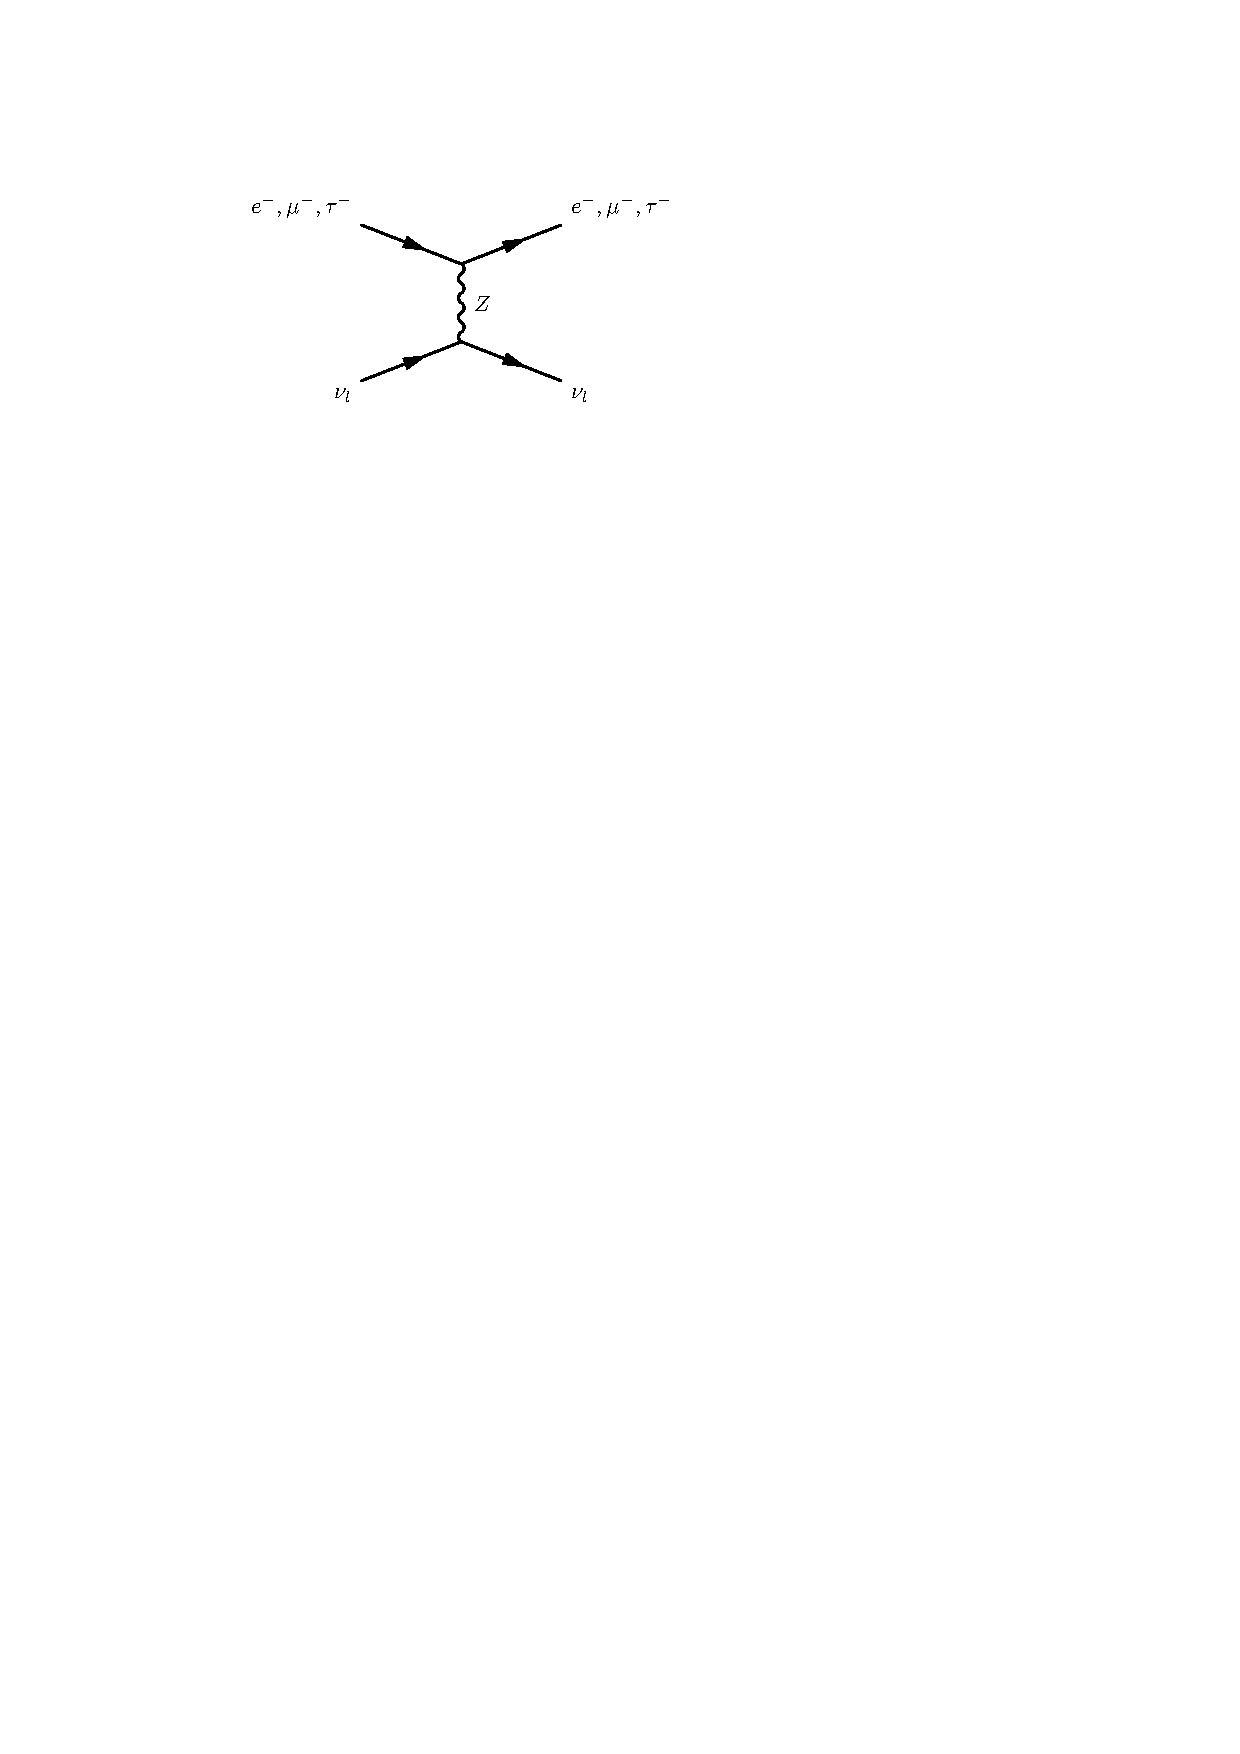
\includegraphics{MatterEffectsNC.pdf}
    \caption{Neutral current scattering.}
    \label{fig:MatterEffectsNC}
  \end{subfigure}
  \hfill
  \begin{subfigure}{0.48\linewidth}
    \centering
    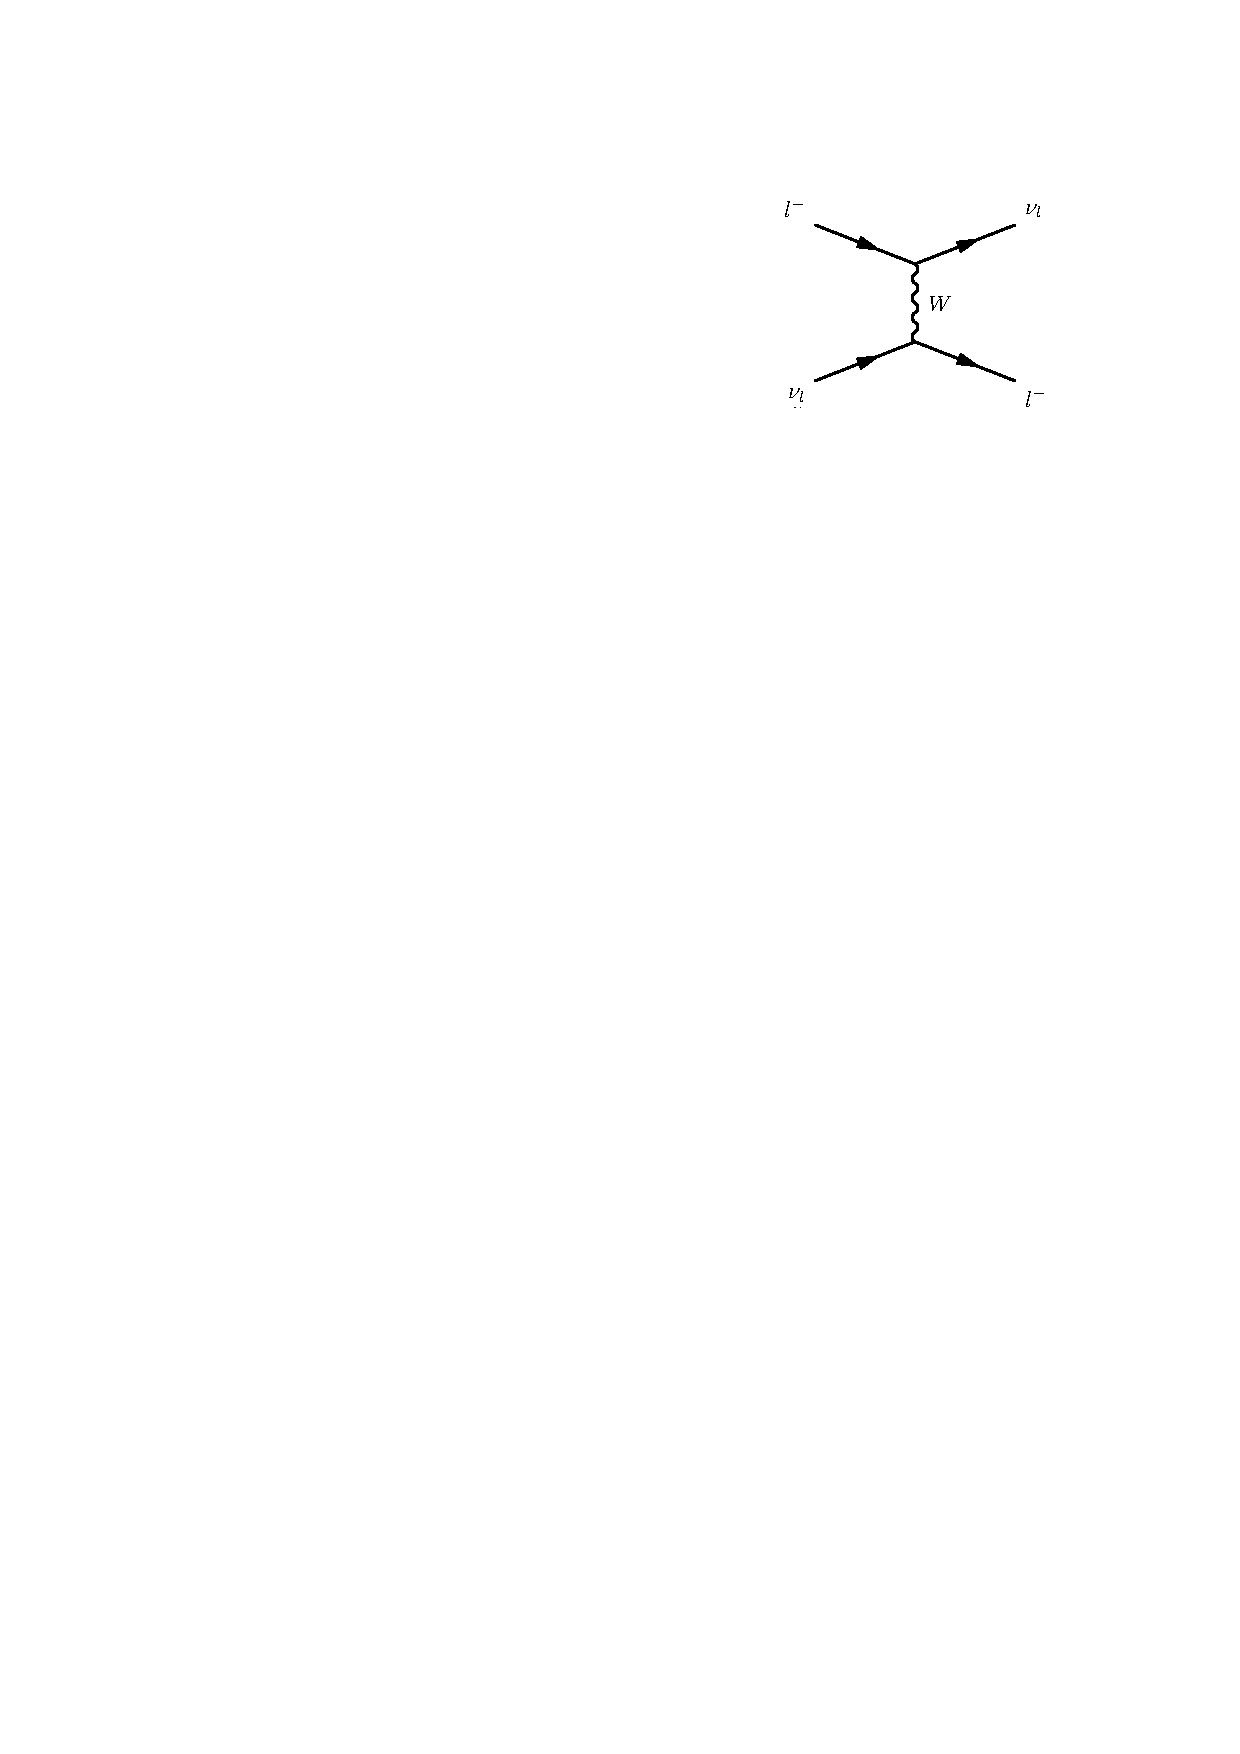
\includegraphics{MatterEffectsCC.pdf}
    \caption{Charged current scattering.}
    \label{fig:MatterEffectsCC}
  \end{subfigure}
  \caption{General scattering mechanics which occur as neutrinos pass through matter.  Neutral current scattering (Figure~\ref{fig:MatterEffectsNC}) occurs for all neutrino flavour combinations whereas charged current scattering (Figure~\ref{fig:MatterEffectsCC}) only occurs when the incoming leptons have the same flavour.}
  \label{fig:MatterEffects}
\end{figure}

\subsubsection{KamLAND and Reactor Neutrinos}\label{sec:KamLAND}

In order to investigate the possible MSW effects in the Sun, measurements of electron neutrino disappearance from terrestrial neutrinos, which were not subject to these matter effects, were considered.  The first experiment to publish results was KamLAND (Kamioka Liquid Scintillator Anti-Neutrino Detector) in 2003 \cite{KamLAND2003,KamLAND2005}.  KamLAND occupied the site previously used by the Kamiokande experiment in Japan under 2700 m.w.e of rock and utilised 1~kton of ultra-pure liquid scintillator contained in a 13~m spherical balloon.  It was surrounded by 53 Japanese nuclear power reactors with baselines ranging from ~80~km to 800~km and detected the $\bar{\nu}_e$s via the inverse beta decay reaction $\bar{\nu}_e + p \rightarrow e^+ + n$.  Scintillation light from the delayed coincidence of a positron with the neutron capture was detected using 1879 PMTs and constituted a signal with very low background.  The results from KamLAND confirmed the apparently large matter effect in solar neutrinos and completely solved for the first time the long-standing Solar Neutrino Problem \cite{Bandyopadhyay2002,deHolanda2002,Fogli2003}.

\subsection{CP Violation}\label{sec:CPViolation}

The $\delta$ terms in Equation~\ref{eq:PMNS} are CP-violating phase factors.  They could be included in any of the diagonalised components but are generally added to the accelerator part since this is how current and future experiments will look for evidence of CP violation.  As long as all the mixing angles are non-zero, there is the possibility of CP violation in the lepton sector.

This is an exciting prospect and one of the reasons for the current intense interest in neutrino physics.  It is known CP-violating processes must have occurred in the early Universe since matter has come to dominate massively over antimatter after they were created equally in the Big Bang.  This has been observed in the quark sector but current experimental evidence can only account for a small amount of the necessary CP violation.  It is also expected but has never been observed in strong interactions \cite{Mannel2007}.  Leptonic CP violation could potentially account for the matter-antimatter asymmetry in the Universe and ultimately explain how it evolved to include our very existence \cite{Ohlsson2012,Ohlsson2013}.

In neutrino experiments, effects of CP violation would be apparent as a difference in behaviour between neutrinos and antineutrinos.  For example, since the sign of $\delta$ is different for neutrinos and antineutrinos, an asymmetry
\begin{equation}\label{eq:NeutrinoAntineutrinoAsymmetry}
  \mathcal{A} = \frac{P(\nu_{\mu}\rightarrow\nu_e)-P(\bar{\nu}_{\mu}\rightarrow\bar{\nu}_e)}{P(\nu_{\mu}\rightarrow\nu_e)+P(\bar{\nu}_{\mu}\rightarrow\bar{\nu}_e)}
\end{equation}
can be observed and measured.

%----------------------------------------------------------------------------------------------------------------------------------------------------------------------------
\section{Status of Neutrino Physics}\label{sec:NeutrinoPhysicsStatus}

The field of neutrino physics has advanced rapidly over the past twenty to thirty years (discussed in Sections \ref{sec:HistoricalContext} and \ref{sec:NeutrinoOscillations}) and there is currently a good understanding of most experimental results in the context of 3-flavour neutrino oscillations.  Presently, the focus has shifted to making precise measurements of the oscillation parameters and trying to understand the nature of neutrino mass.  The current understanding of each of these areas will be presented in Sections \ref{sec:OscillationParameters} and \ref{sec:NeutrinoMass} respectively following a brief overview of current and future experiments in Section~\ref{sec:CurrentExperiments}.

%----------------------------------------------------------------------------------------------------------------------------------------------------------------------------
\subsection{Current and Future Experiments}\label{sec:CurrentExperiments}

In recent years, neutrino experiments which utilise a custom built artificial neutrino beam have been offering complimentary and world-leading results.  These `accelerator experiments' are used in order to have more control over the energy spectrum and composition of the neutrino beam and often use a long-baseline, sampling the beam at different points to determine the effects of oscillation as the neutrinos propagate in between.

MINOS was based at Fermilab, U.S., and detected neutrinos from the NuMI (Neutrinos at the Main Injector) beam at a `near detector' and then again in Northern Minnesota, a baseline of 735~km.  T2K follows a similar design and uses the Super-Kamiokande detector as the far detector, utilising a beam from J-PARC, Japan and a baseline of 295~km.  T2K and NO$\nu$A, another current long-baseline experiment, were designed specifically to measure the last mixing parameter, $\theta_{13}$, by looking for $\nu_e$ appearance in a $\nu_{\mu}$ beam.  NO$\nu$A, like its predecessor MINOS, also uses the NuMI beam and has a far detector at the same site.  However, along with T2K, it is `off-axis' by around $2^{\circ}$; this produces a more monotonic neutrino energy spectrum to maximise the effect of oscillations and make more accurate measurements.  T2K and NO$\nu$A still have many years left of their respective programmes and are currently making precision measurements of the mixing parameters along with constraining CP violation by combining neutrino and antineutrino analyses.  They will not be able to make statistically significant measurements of this area but, especially through joint analyses, will be able to offer hints before the next generation of experiments.

Future long-baseline experiments include DUNE \cite{DUNECDR1}, which will be discussed properly in Chapter \ref{chap:DUNE}, and Hyper-Kamiokande \cite{HyperKamiokande2015}, an upgrade of the current T2K experiment.  Hyper-Kamiokande will also use water Cherenkov technology but will boast a fiducial volume 25 times larger than that of Super-Kamiokande.  The timescale of these projects is on the order of at least ten years from now and both pose incredible engineering challenges in their own right.

%----------------------------------------------------------------------------------------------------------------------------------------------------------------------------
\subsection{Oscillation Parameters}\label{sec:OscillationParameters}

The current status of the mixing angles and the mass-squared differences is depicted in Figure~\ref{fig:GlobalFit}.  The world-best measurements for $\theta_{12}$ and $\Delta m^2_{12}$ are provided by the solar neutrino experiments (Homestake \cite{Cleveland1995}, GALLEX \cite{Gallex2010}, SAGE \cite{Sage2009} and SNO \cite{SNO2013}) and KamLAND \cite{KamLAND2013}.  The leading measurements in the atmospheric neutrino sector, $\theta_{23}$ and $|\Delta m_{32}^2|$, are from Super-Kamiokande \cite{SuperKamiokande2010}, IceCube \cite{IceCube2015} and the accelerator experiments MINOS \cite{MINOS2013,MINOS2013b}, T2K \cite{T2Knumu2014} and NO$\nu$A \cite{NOvAnumu2016}.

\begin{figure}[p]
  \centering
  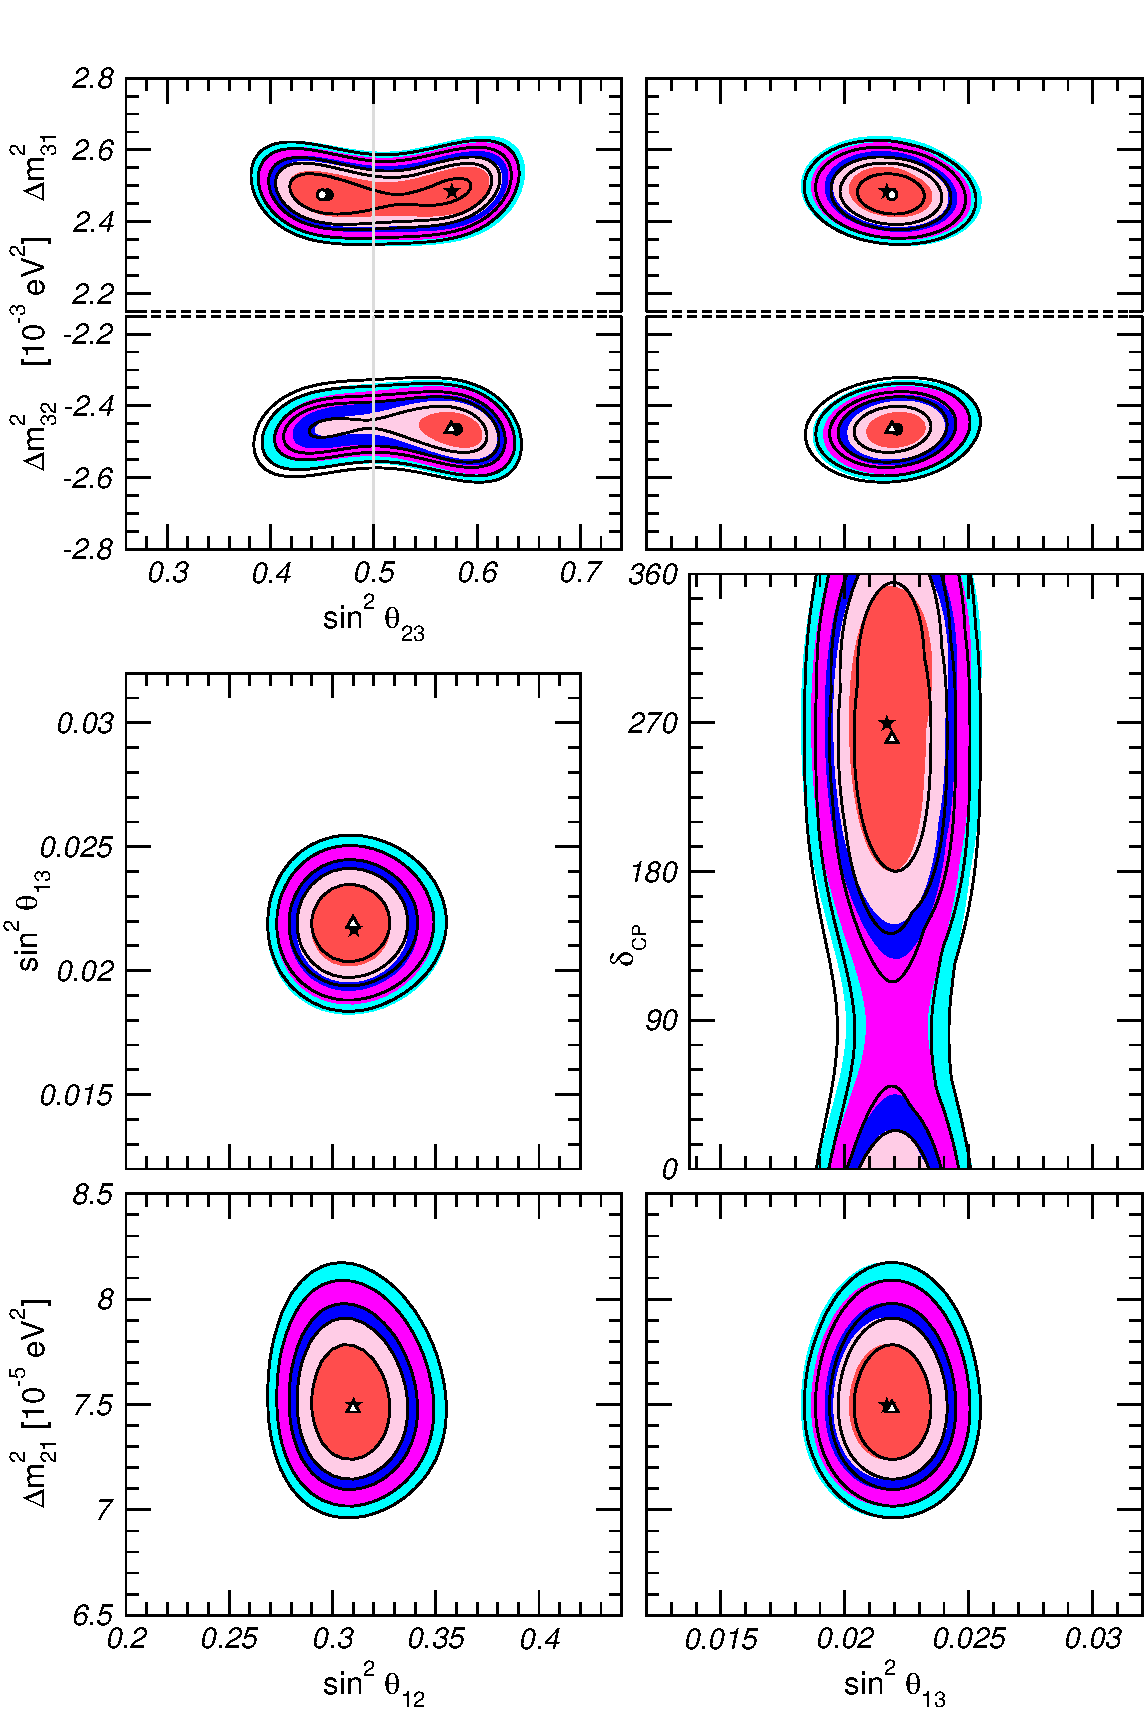
\includegraphics[width=12cm]{GlobalFit.pdf}
  \caption{Global 3-neutrino oscillation analysis taken from \cite{NuFit2014,NuFit2017}. Each panel shows the two-dimensional projection of the allowed six-dimensional region after marginalisation with respect to the undisplayed parameters. The different contours correspond to 1$\sigma$, 90\%, 2$\sigma$, 99\%, 3$\sigma$ CL (2 dof).}
  \label{fig:GlobalFit}
\end{figure}

The value of $\theta_{13}$ was known, from limits determined from global fits to world data, to be much smaller than the others and was even consistent with zero.  In addition to the accelerator experiments, reactor neutrino experiments are also sensitive to $\theta_{13}$ via $\bar{\nu}_e$ disappearance and it was these experiments which produced the decisive results first.  Daya Bay \cite{DayaBay2012} in China and RENO \cite{RENO2012} in South Korea found evidence of a non-zero value in 2012.  There is good agreement between these reactor experiments and more recent measurements from T2K \cite{T2Knue2014} and NO$\nu$A \cite{NOvAnue2016}.

A summary of the best known values for all these oscillation parameters is shown in Table \ref{tab:OscillationParameters}.  The CP-violating phase $\delta_{\textnormal{CP}}$ is currently unmeasured and provides a priority for current and future neutrino experiments.  T2K have excluded the CP conservation regions with little statistical significance and currently favours a maximal CP violation value of $\delta_{\textnormal{CP}} = -\pi/2$ \cite{T2K2017}; this holds much promise for future experiments.  The octant of $\theta_{23}$, the location of the parameter in either the $> 45^{\circ}$ or $< 45^{\circ}$ octant, is also undetermined and requires high precision measurements; it is possible that the mixing in this sector is `maximal' ($\theta_{23} = 45^{\circ}$).

\begin{table}
  \caption{The current best-fit values for the neutrino oscillation parameters for normal (inverted) hierarchy.  Taken from \cite{NuFit2017}.}
  \label{tab:OscillationParameters}
  \centering
%  \resizebox*{\columnwidth}{!}{
    \begin{tabular}{c c}
      \toprule
      Parameter & Best fit ($\pm 1\sigma$) \\
      \midrule
      $\sin^2{\theta_{12}}$ & $0.306\pm0.012$ \\
      $\sin^2{\theta_{23}}$ & $0.441^{+0.027}_{-0.021}$ ($0.587^{+0.020}_{-0.024}$) \\
      $\sin^2{\theta_{13}}$ & $0.02166\pm0.00075$ ($0.02179\pm0.00076$) \\
      \midrule
      $\Delta m_{12}^2$ [$10^{-5}$~eV$^2$]     & $+7.50^{+0.19}_{-0.17}$ \\
      $|\Delta m_{3\nu}^2|$ [$10^{-3}$~eV$^2$] & $2.524^{+0.039}_{-0.040}$ ($-2.514^{+0.038}_{-0.041}$) \\
      \midrule
      $\delta_{\textnormal{CP}}$ [$^{\circ}$] & $261^{+51}_{-59}$ ($277^{+40}_{-46}$) \\
      \bottomrule
    \end{tabular}
 % }
\end{table}

%----------------------------------------------------------------------------------------------------------------------------------------------------------------------------
\subsection{Neutrino Mass}\label{sec:NeutrinoMass}

Neutrinos in the Standard Model are massless, for no real reason.  However, the observation of neutrino oscillations implies the existence of neutrino mass (the oscillation probabilities, such as Equations~\ref{eq:ElectronNeutrinoAppearance} and~\ref{eq:MuonNeutrinoDisappearance}, would be zero if there was no mass splitting).  Three active neutrino flavours gives rise to two independent mass splittings, $\Delta m_{12}^2$ and $\Delta m_{32}^2$, as appear in the oscillation probabilities.  Unfortunately, fitting to the oscillation results provides only a handle on the value of these splittings and not the signs, resulting in an ambiguity in the ordering of the mass states.  This can be resolved in the solar sector by utilising the effect of the MSW resonance encountered by neutrinos in the Sun, allowing the sign of $\Delta m_{12}^2$ to be known (it must be positive as otherwise fewer oscillations, not more, will have been observed by SNO and the other solar neutrino experiments).  This leaves two possible `hierarchies', normal and inverted, which are possible given the experimental data.  These mass splittings also do not offer any indication of an absolute mass scale for the neutrino mass states, this must be constrained using other methods and is currently undetermined.  These uncertainties are illustrated in Figure~\ref{fig:MassHierarchy}.

\begin{figure}
  \centering
  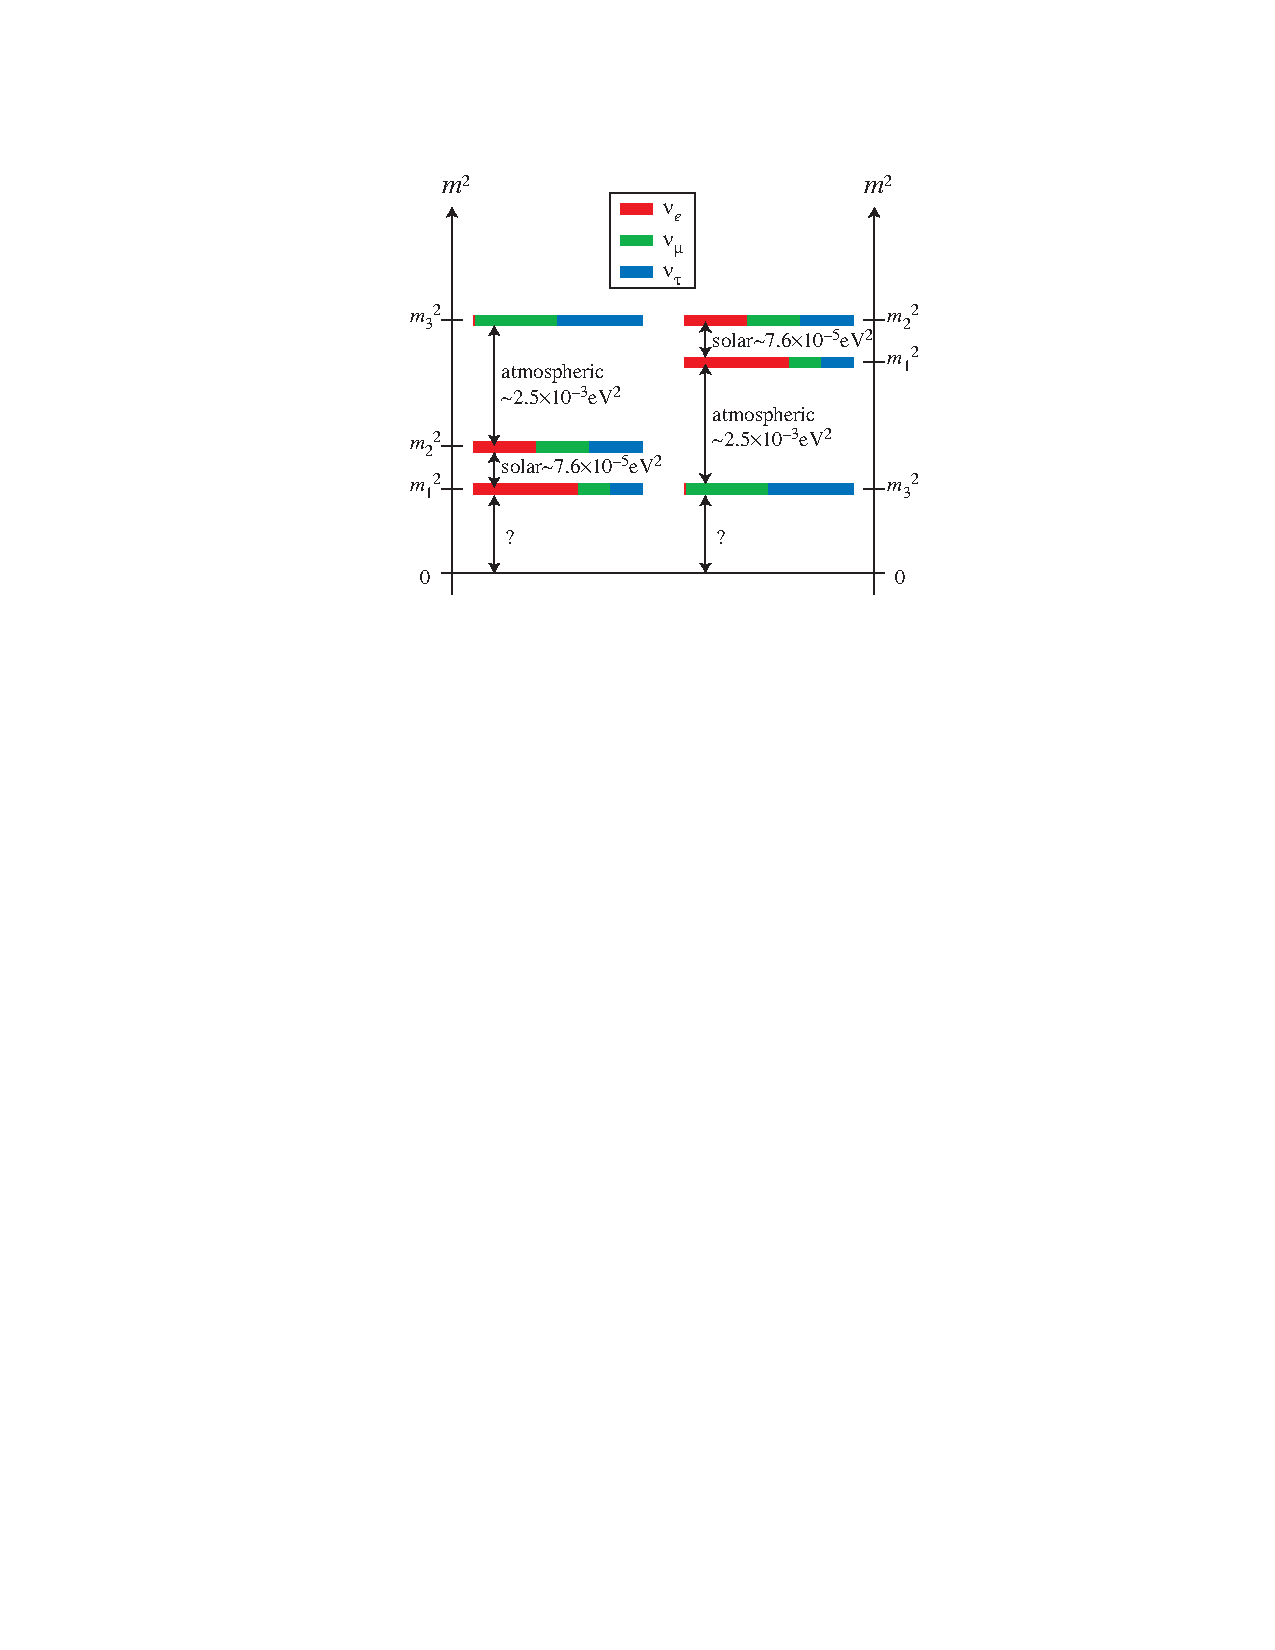
\includegraphics[width=10cm]{MassHierarchy.pdf}
  \caption[Demonstration of the current uncertainties in the neutrino mass.]{Demonstration of the current uncertainties in the neutrino mass.  The undetermined sign in the mass splitting between the 2 and 3 states leaves two possible `hierarchies' open: normal (left figure) and inverted (right figure).  The absolute scale of the masses is also currently unknown.  The flavour composition of each of the mass states, given by the mixing angles, is denoted by the coloured bars.}
  \label{fig:MassHierarchy}
\end{figure}

DUNE will use the MSW effect present as neutrinos propagate through the Earth's crust in order to resolve the hierarchy problem.  It is essential that the hierarchy is resolved since the associated asymmetries between neutrinos and antineutrinos can mimic true CP violation, which therefore cannot be measured accurately until the mass splittings are completely understood.  Due to the large matter effects associated with its long baseline, the NO$\nu$A experiment is sensitive to the mass hierarchy and may be able to have a say before DUNE and Hyper-Kamiokande.

The absolute neutrino mass cannot be measured from oscillation experiments so other techniques have been developed.  It is possible to use information from $\beta$-decay to get a handle on the mass scale; the $\bar{\nu}_e$ mass alters the spectrum of electrons near the end point so precision measurements can study this effect.  The current best limits on the mass are from H$^3$ $\beta$-decay experiments and yield $m_{\bar{\nu}_e} < 2.05$~eV at 95\% C.L. \cite{Triotsk2011,Mainz2005}.  Cosmological analysis can also constrain the absolute neutrino mass by looking at the distribution of matter in the Universe and information such as galaxy clustering.  The Planck collaboration reported the upper limit on the sum of all neutrino masses as $\sum_i m_{\nu_i} < 0.23$~eV at 95\% C.L. in 2013 \cite{Planck2013}, indicating a significantly lower mass scale than is attainable using current experiments.
